\documentclass{beamer}
\usetheme{Warsaw}



\setbeamercolor{normal text}{fg=white,bg=black!90}
\setbeamercolor{structure}{fg=white}

\setbeamercolor{alerted text}{fg=red!85!black}

\setbeamercolor{item projected}{use=item,fg=black,bg=item.fg!35}

\setbeamercolor*{palette primary}{use=structure,fg=structure.fg}
\setbeamercolor*{palette secondary}{use=structure,fg=structure.fg!95!black}
\setbeamercolor*{palette tertiary}{use=structure,fg=structure.fg!90!black}
\setbeamercolor*{palette quaternary}{use=structure,fg=structure.fg!95!black,bg=black!80}

\setbeamercolor*{framesubtitle}{fg=white}

\setbeamercolor*{block title}{parent=structure,bg=black!60}
\setbeamercolor*{block body}{fg=black,bg=black!10}
\setbeamercolor*{block title alerted}{parent=alerted text,bg=black!15}
\setbeamercolor*{block title example}{parent=example text,bg=black!15}


\setbeamertemplate{navigation symbols}{}


\begin{document}


{
    \usebackgroundtemplate
    {
        \vbox to \paperheight{\vfil\hbox to \paperwidth{\hfil

        {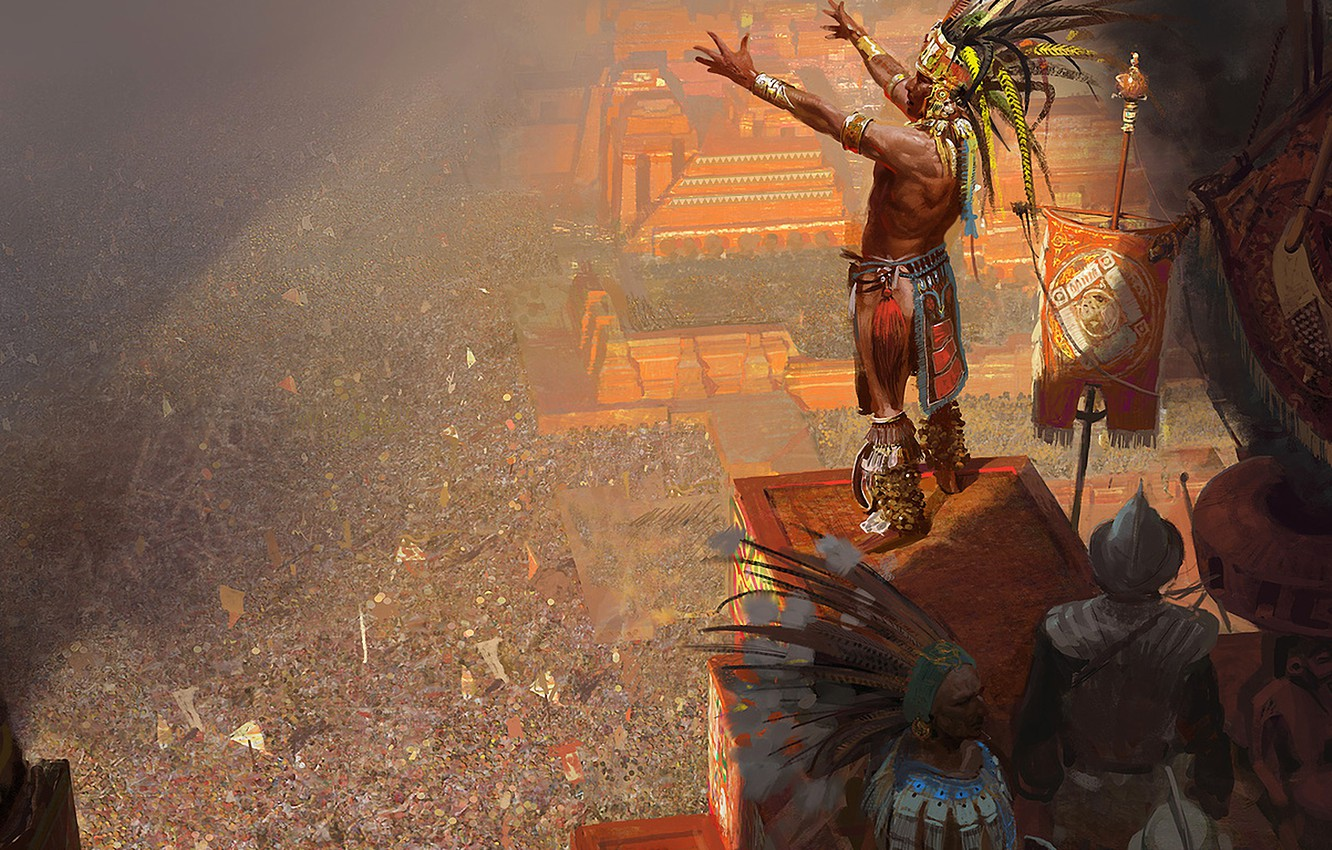
\includegraphics[width=5.05in]{../images/aztec.jpg}}

        \hfil}\vfil}
    }

    \begin{frame}
     \centering
     {
        \begin{minipage}{10cm}
           {\LARGE \color{white}{\bf Exploration by \\ self supervised-exploitation}} \\ \\
           {\LARGE \color{white}{\bf Matej Pecháč}} \\
           {\LARGE \color{white}{\bf Michal Chovanec}} \\
           {\LARGE \color{white}{\bf Igor Farkaš}} \\ \\ 
           {\color{white}{Department of Applied Informatics}} \\
           {\color{white}{Comenius University in Bratislava}} \\
           {\color{white}{Slovak Republic}}
       \end{minipage}
     }

    \end{frame}
}

\begin{frame}
  \frametitle{Exploration by self supervised-exploitation}
  
  \centering
  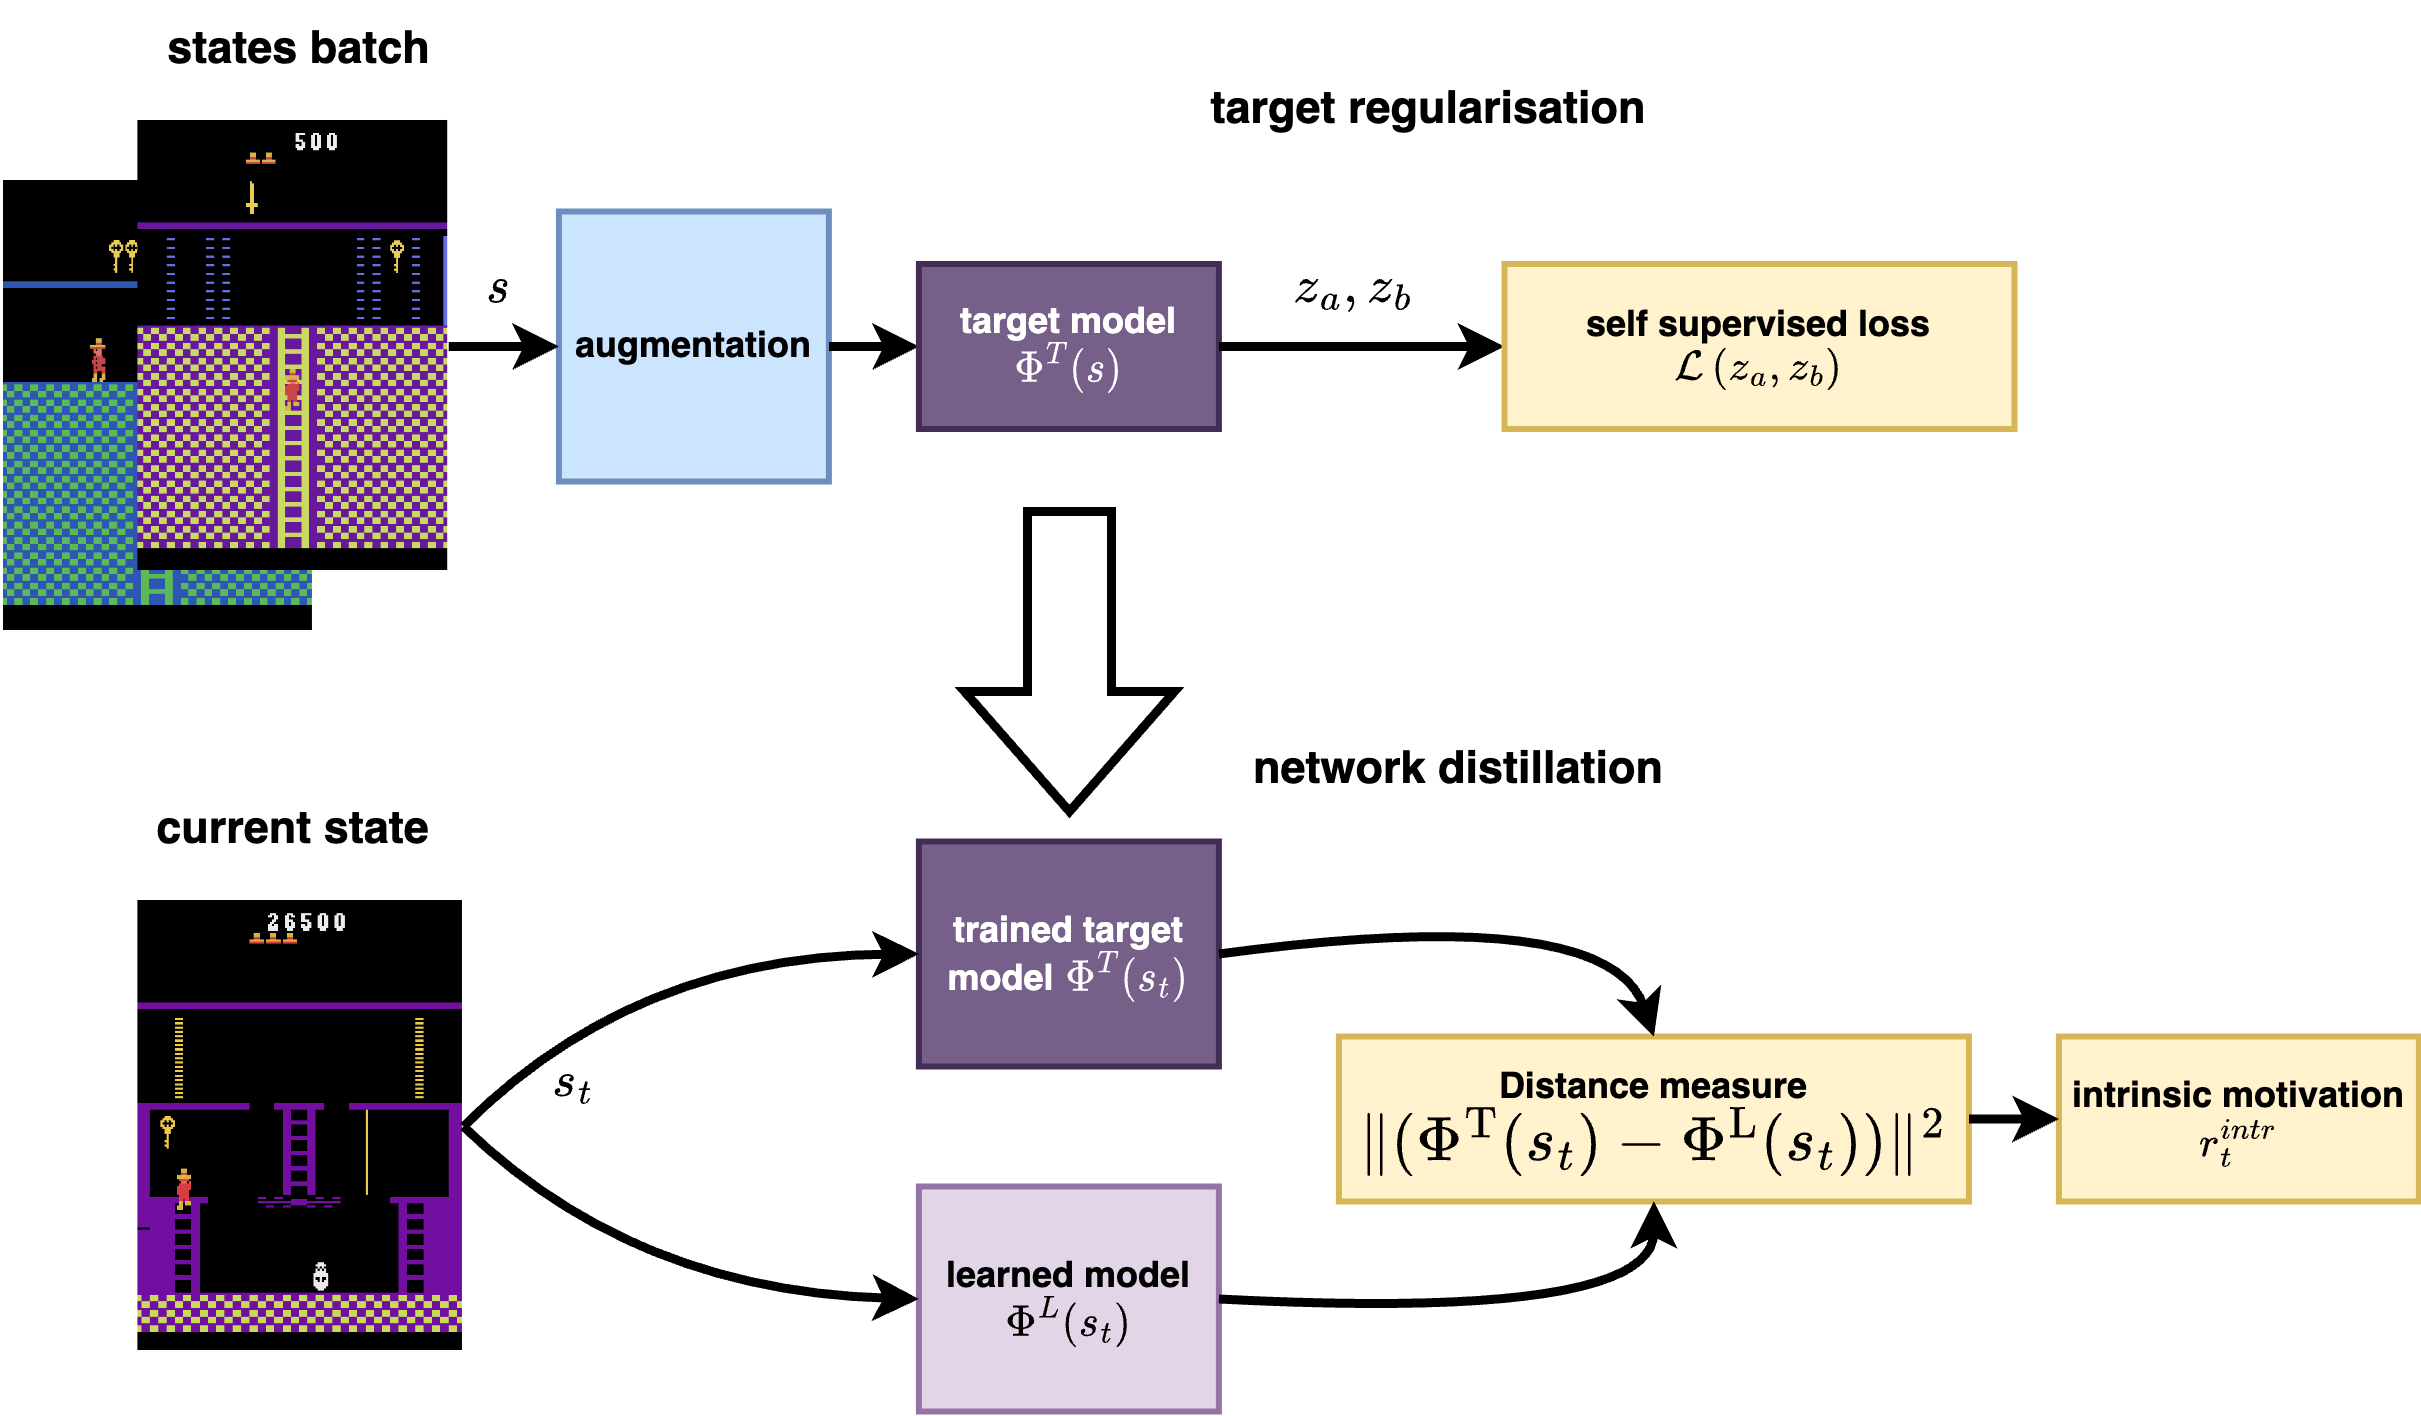
\includegraphics[scale=0.5]{../diagrams/cnd/cnd-cnd.png}

\end{frame}


\begin{frame}
  \frametitle{Exploration by self supervised-exploitation}

  \vskip 0pt plus 1filll
    \centering
    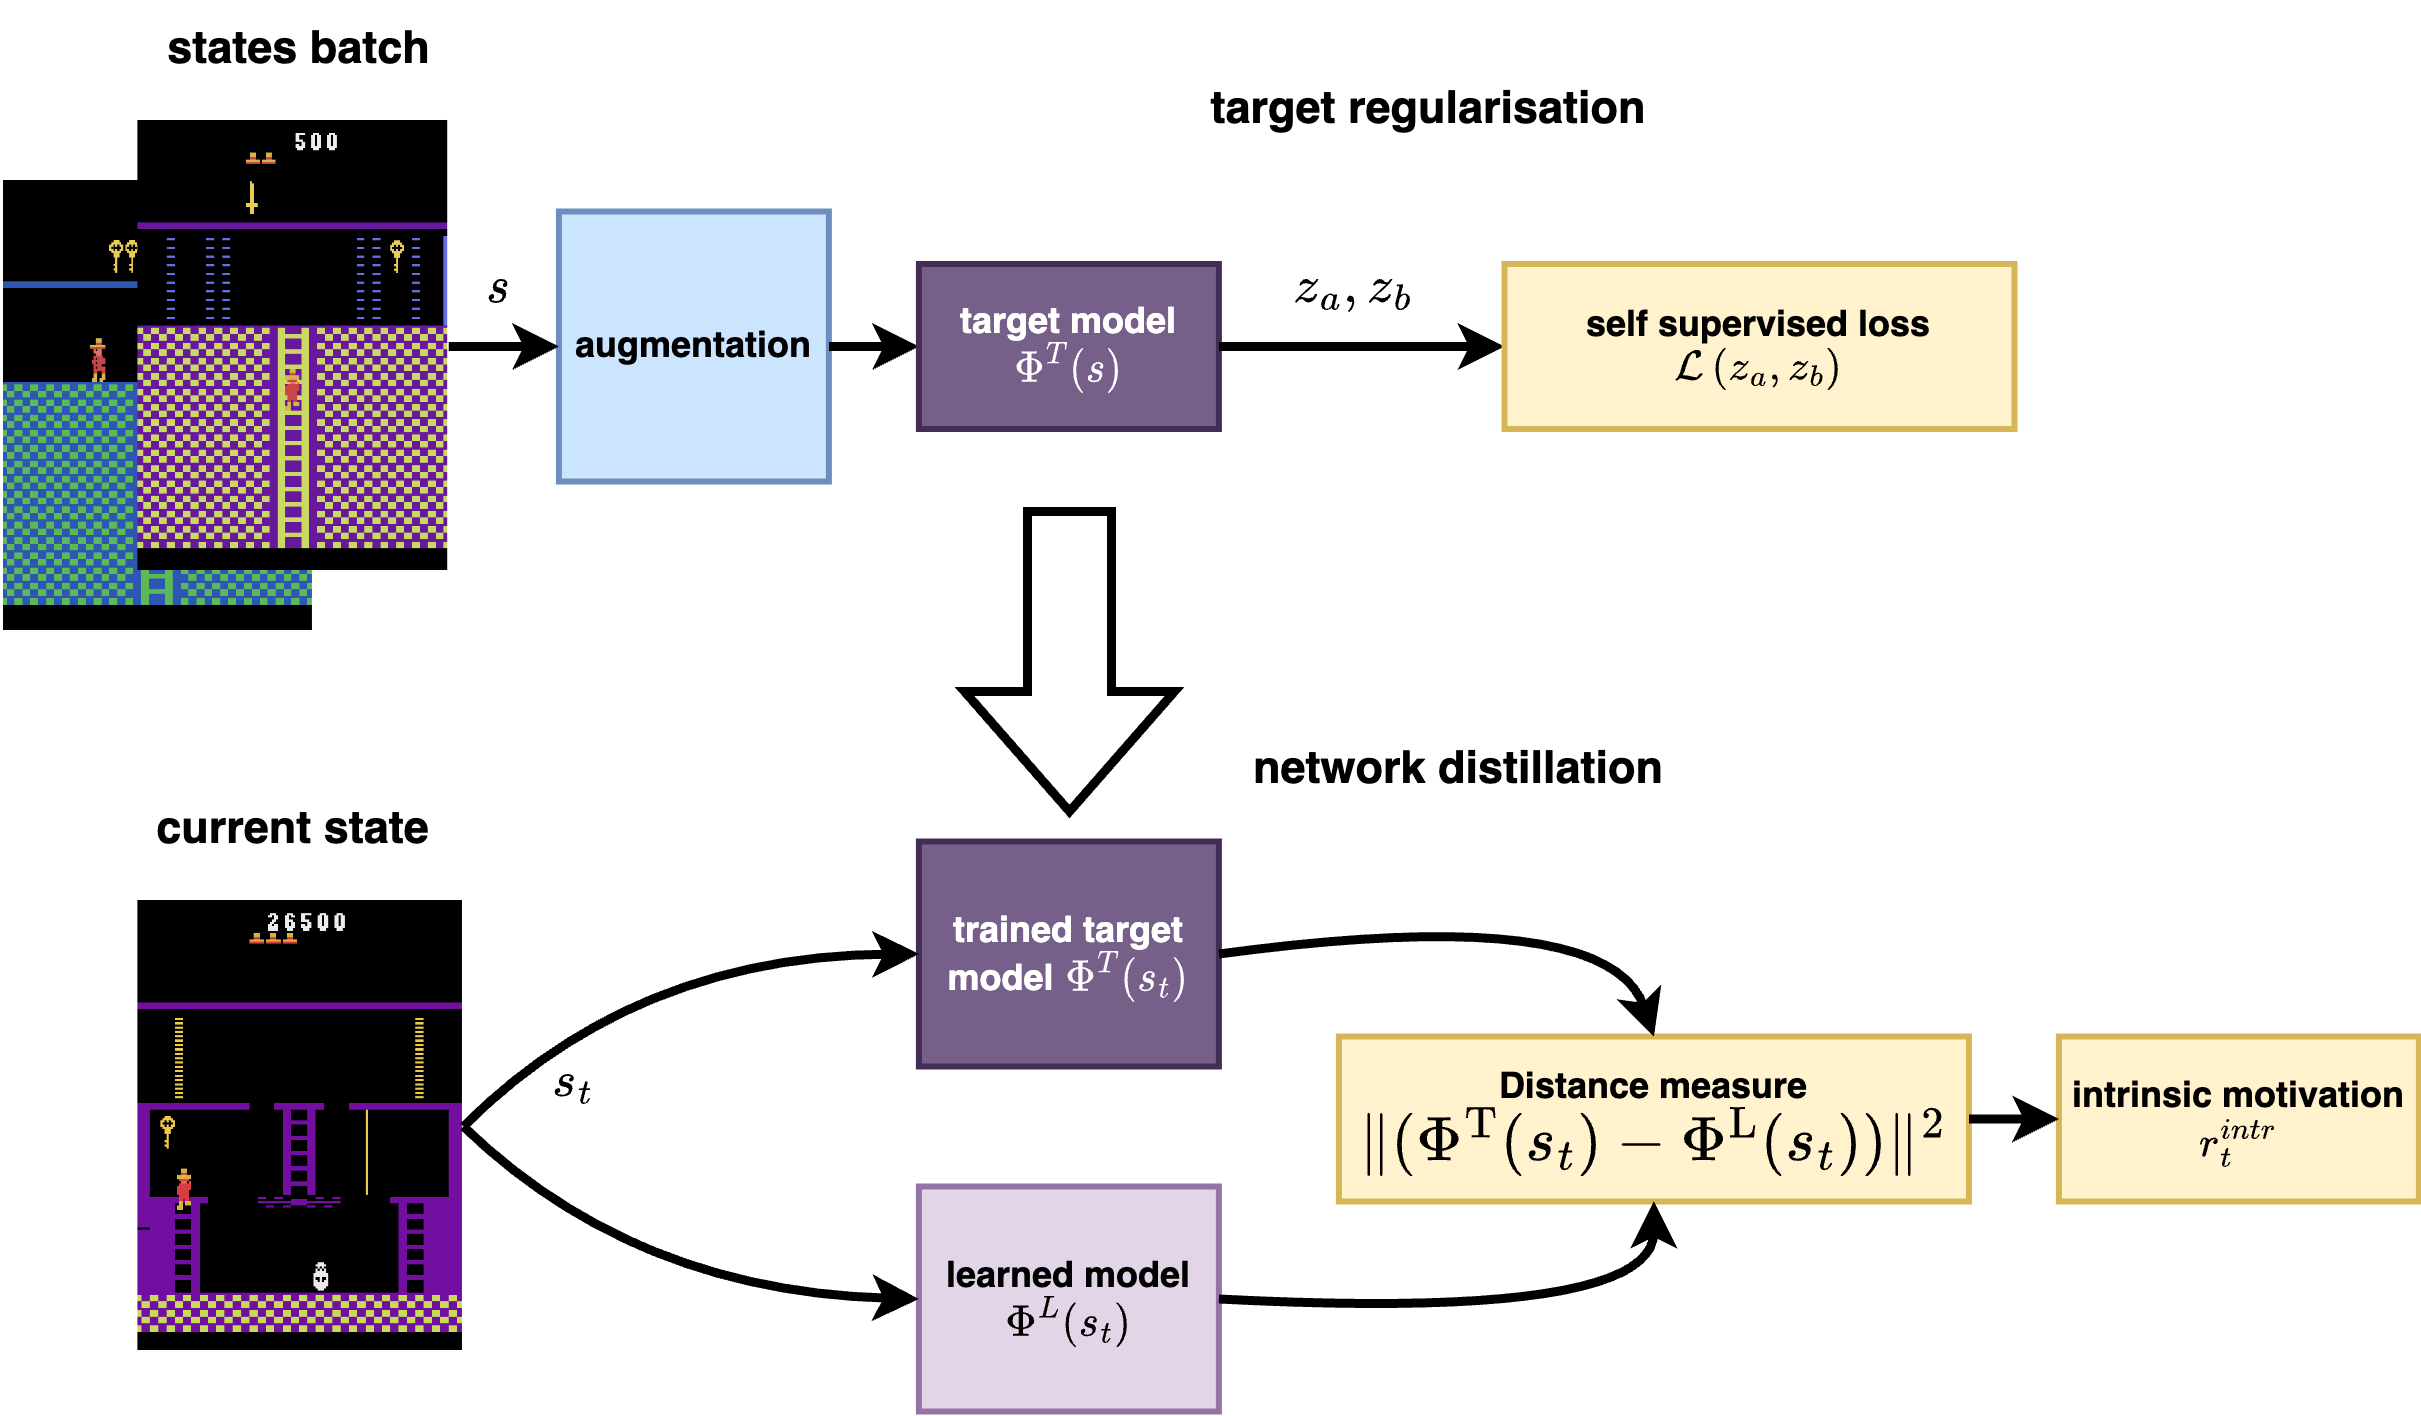
\includegraphics[scale=0.4]{../diagrams/cnd/cnd-cnd.png}

\end{frame}

\begin{frame}
  \frametitle{Exploration by self supervised-exploitation}

  \begin{itemize}
    \item we extended existing idea of Random Network Distillation
  \end{itemize}

  \vskip 0pt plus 1filll
    \centering
    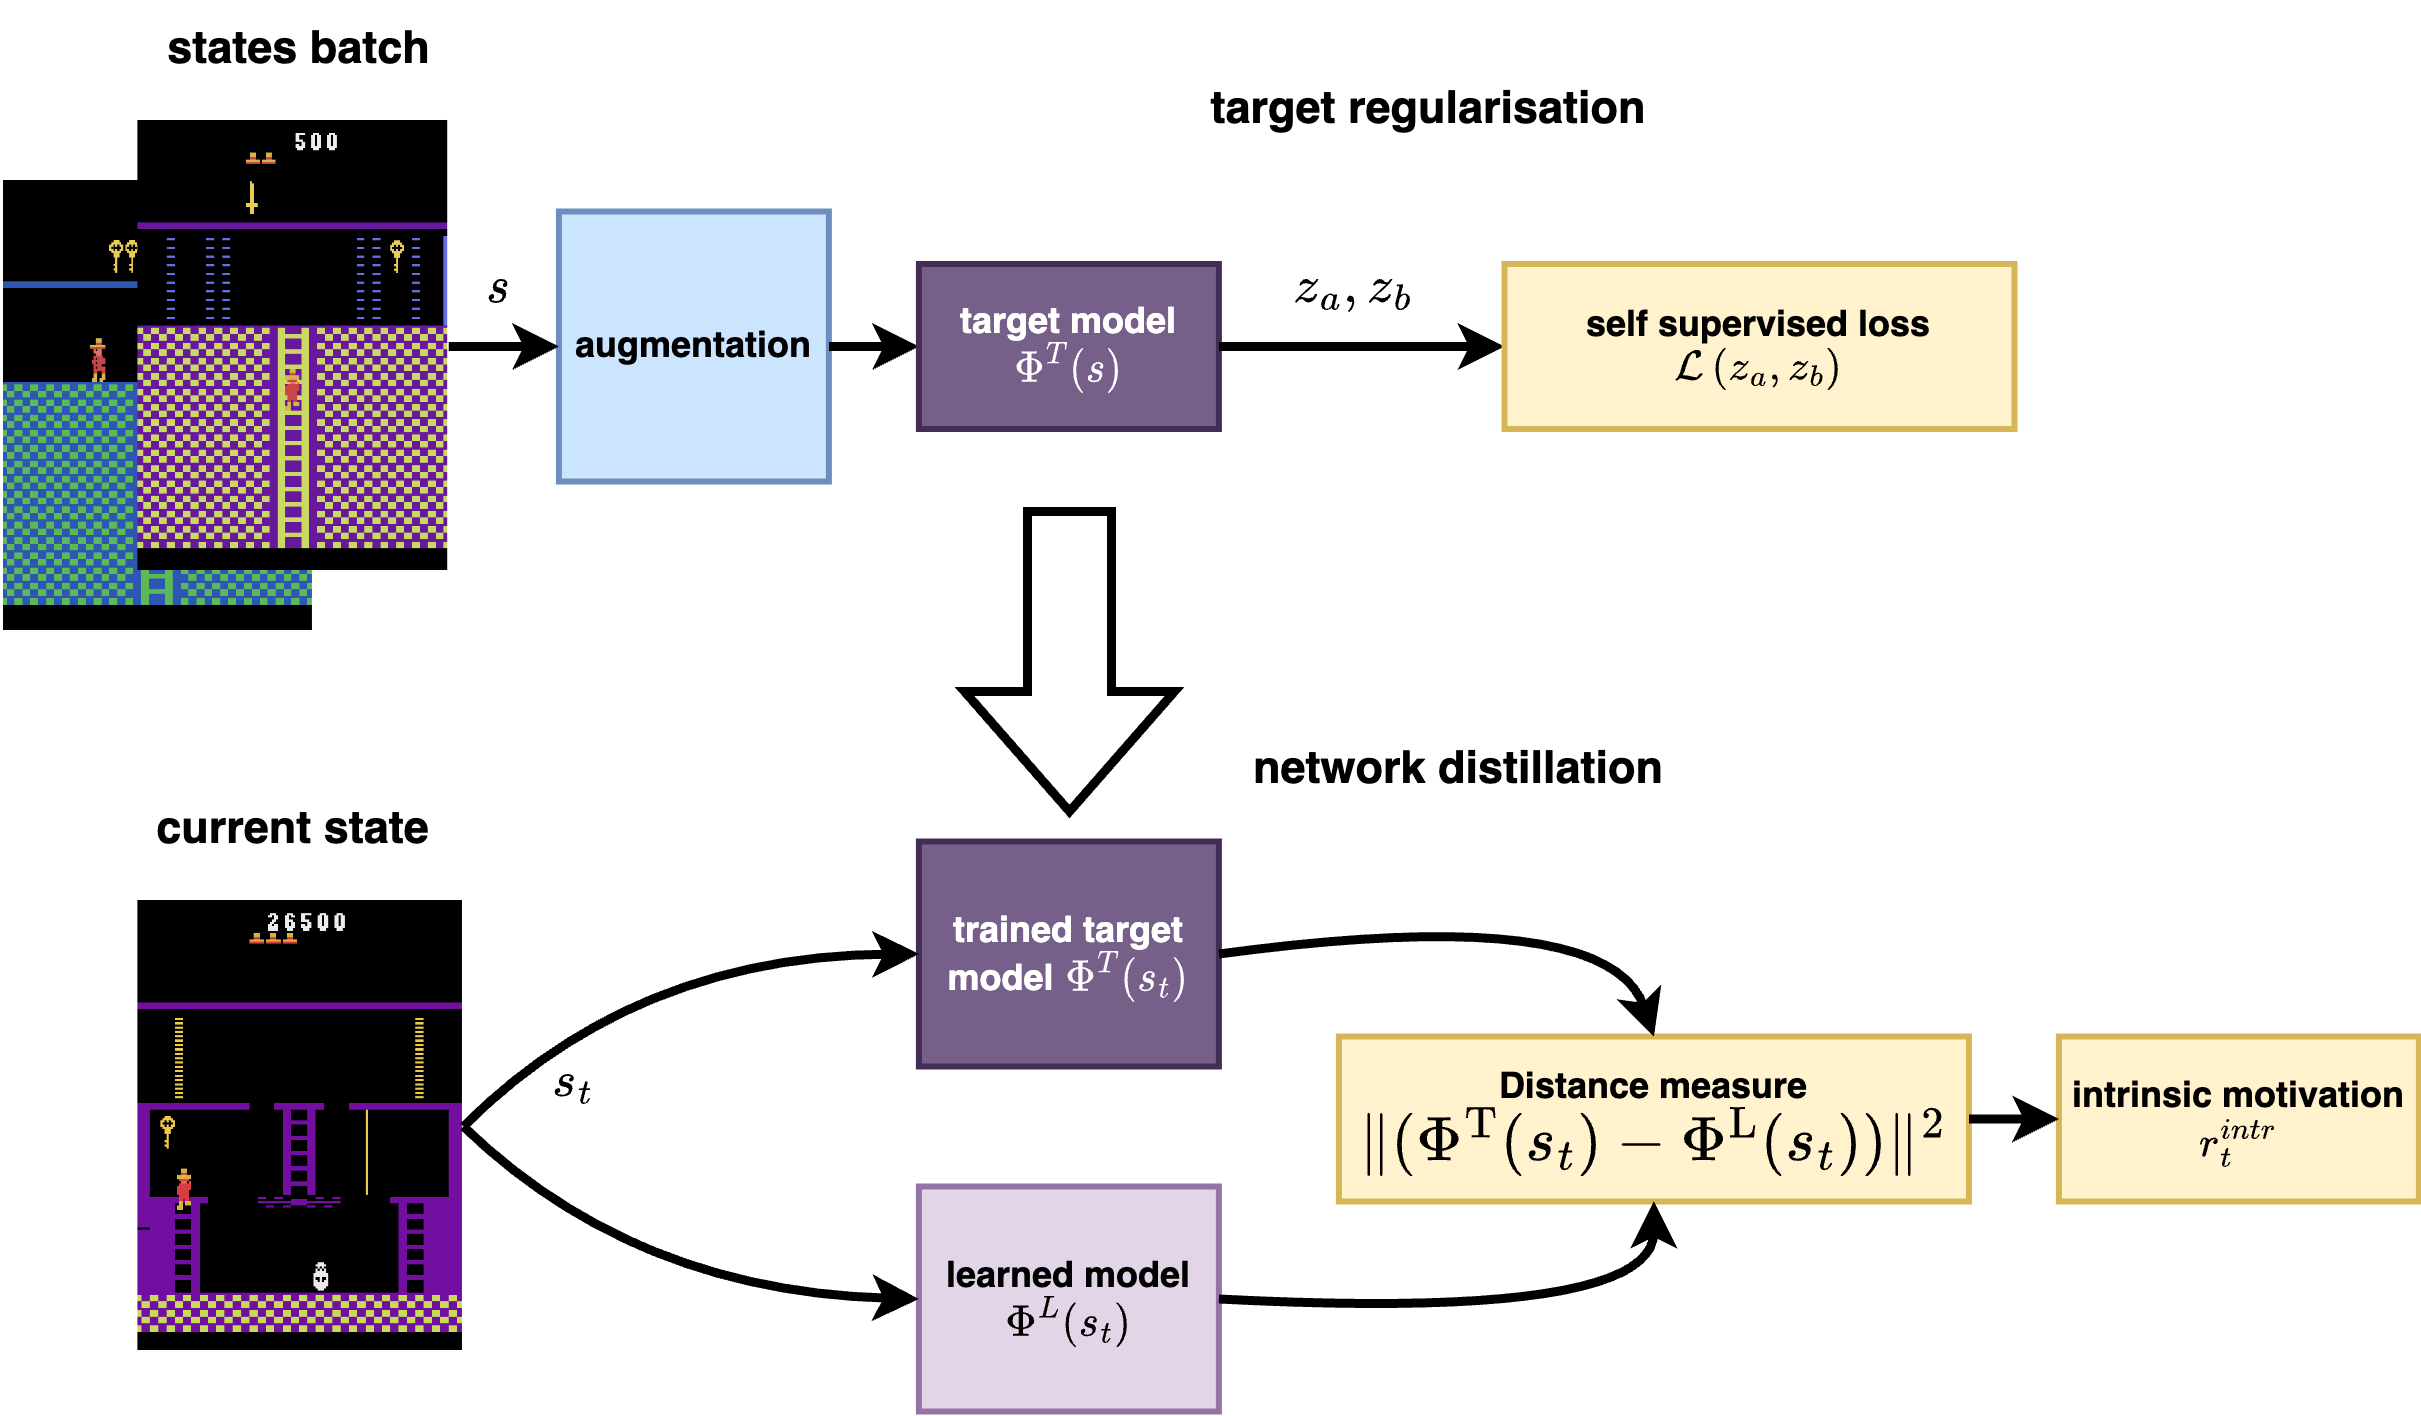
\includegraphics[scale=0.4]{../diagrams/cnd/cnd-cnd.png}

\end{frame}


\begin{frame}
  \frametitle{Exploration by self supervised-exploitation}

  \begin{itemize}
    \item we extended existing idea of Random Network Distillation
    \item {\color{red} 1 : } for target model, self supervised training is used
  \end{itemize}

  \vskip 0pt plus 1filll
    \centering
    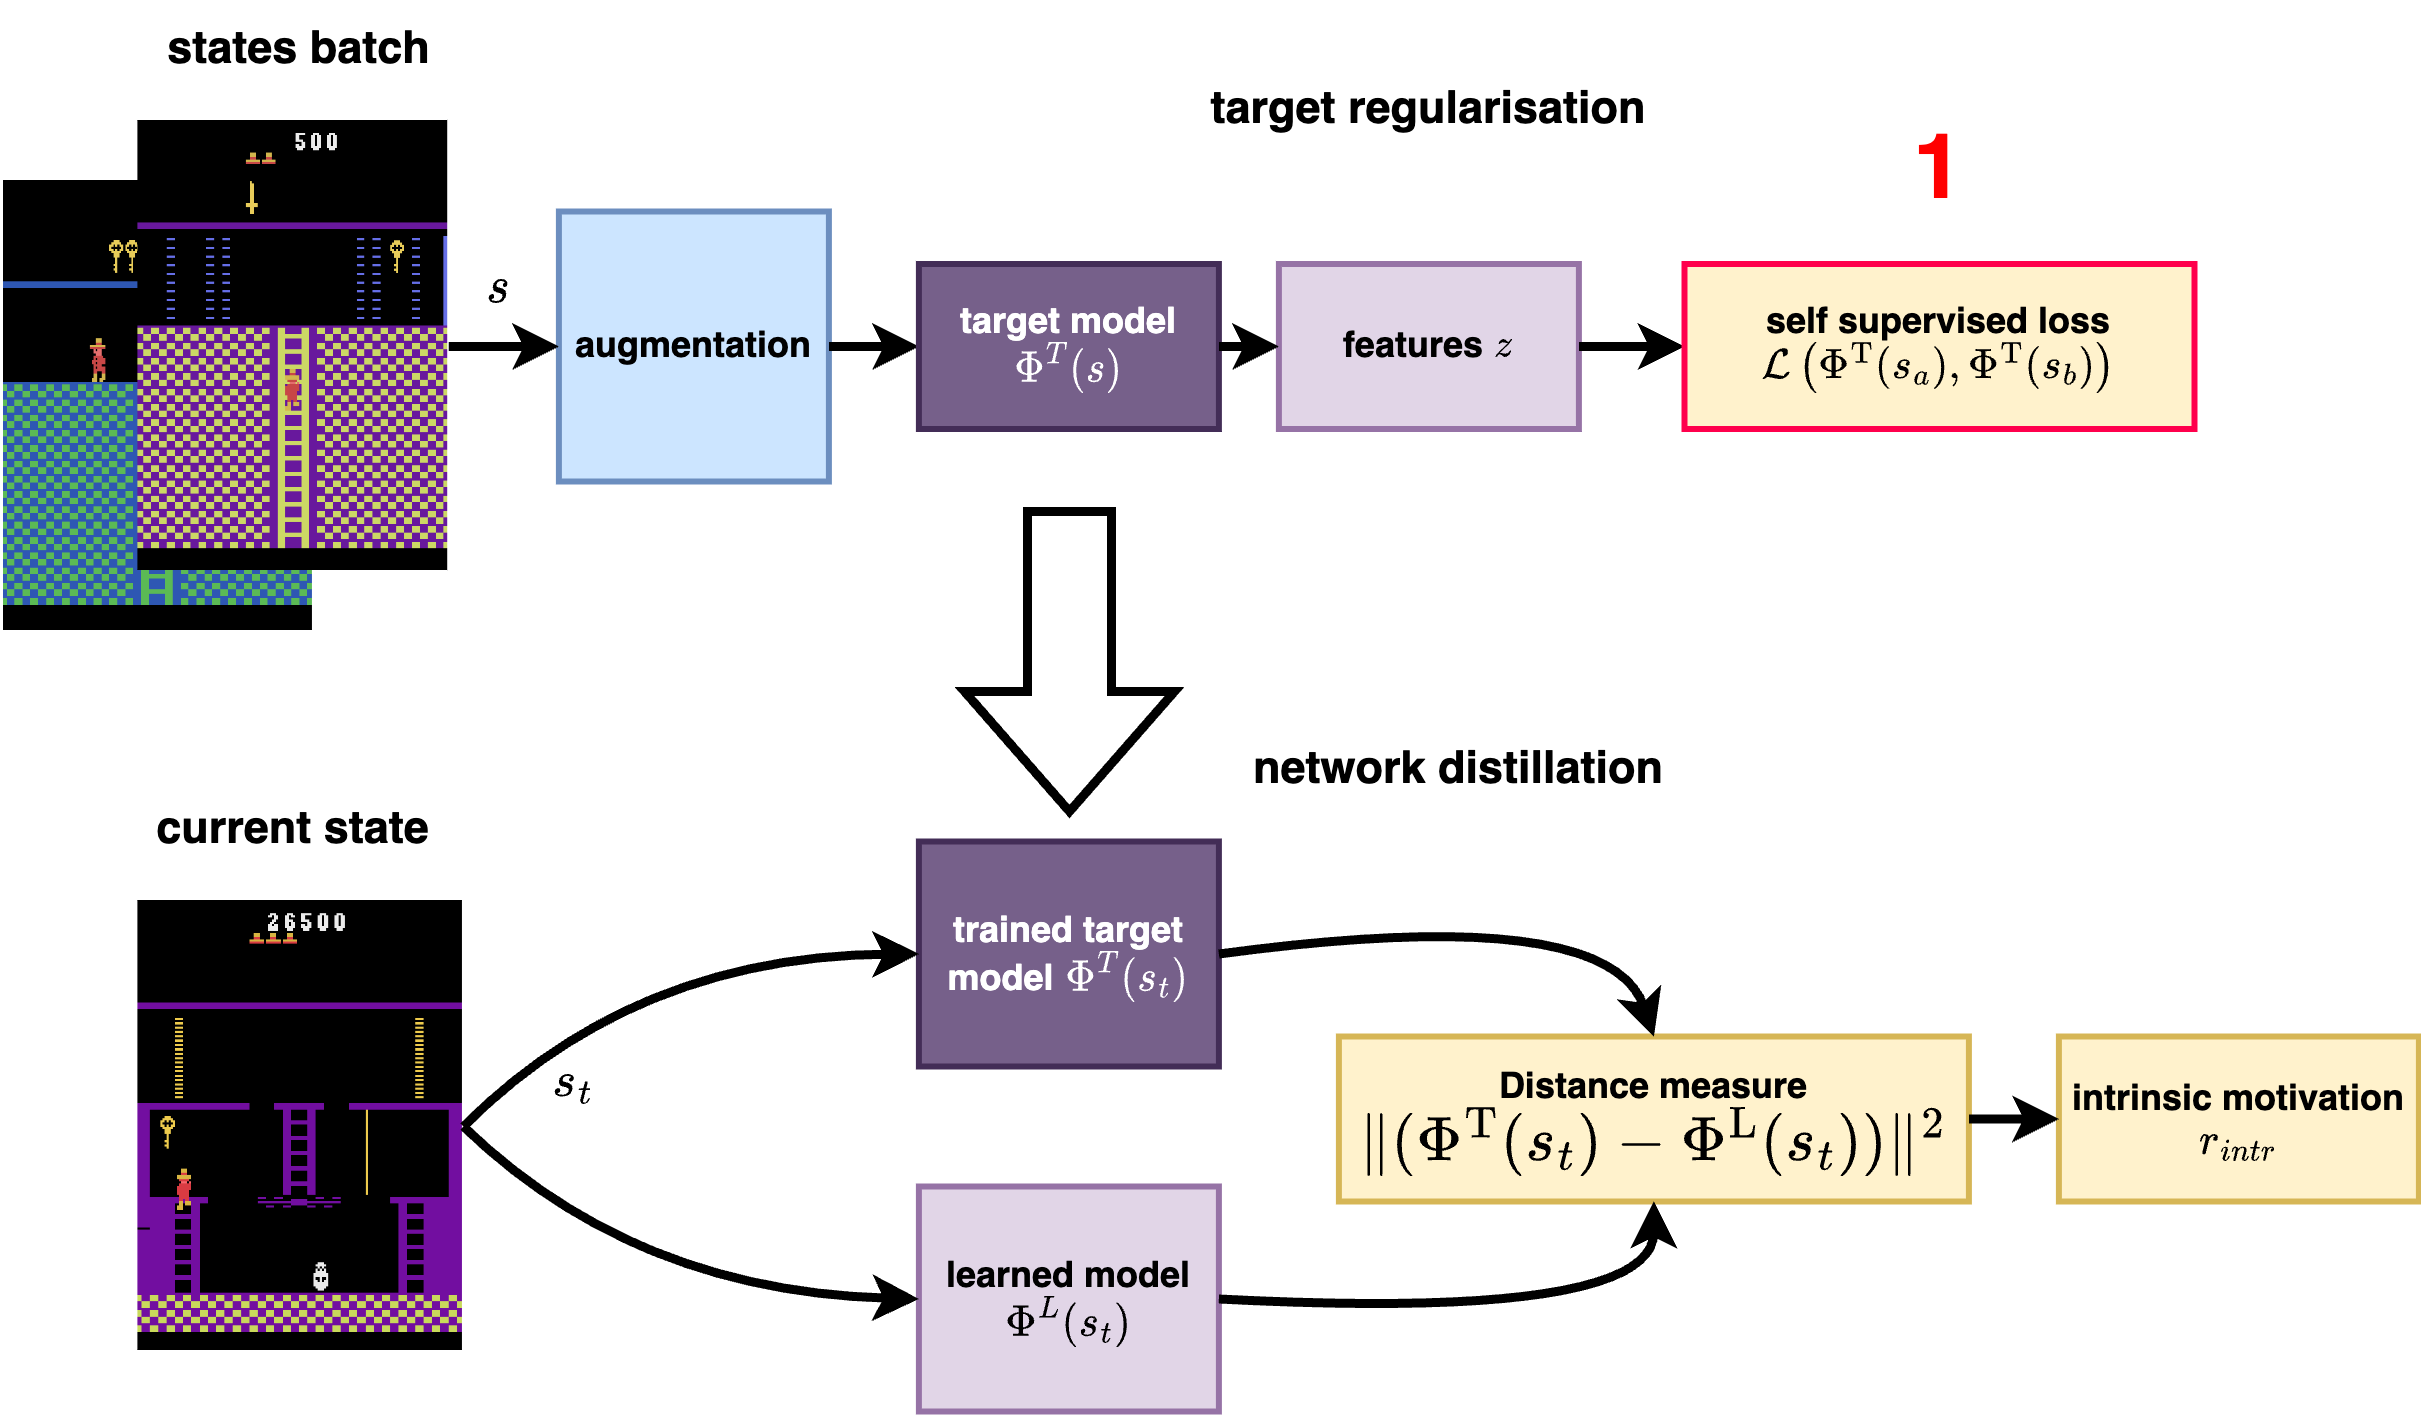
\includegraphics[scale=0.4]{../diagrams/cnd/cnd-cnd-1.png}

\end{frame}

\begin{frame}
  \frametitle{Exploration by self supervised-exploitation}

  \begin{itemize}
    \item we extended existing idea of Random Network Distillation
    \item {\color{red} 1 : } for target model, self supervised training is used
    \item {\color{red} 2 : } augmented states are used to train target model
  \end{itemize} 

  \vskip 0pt plus 1filll
    \centering
    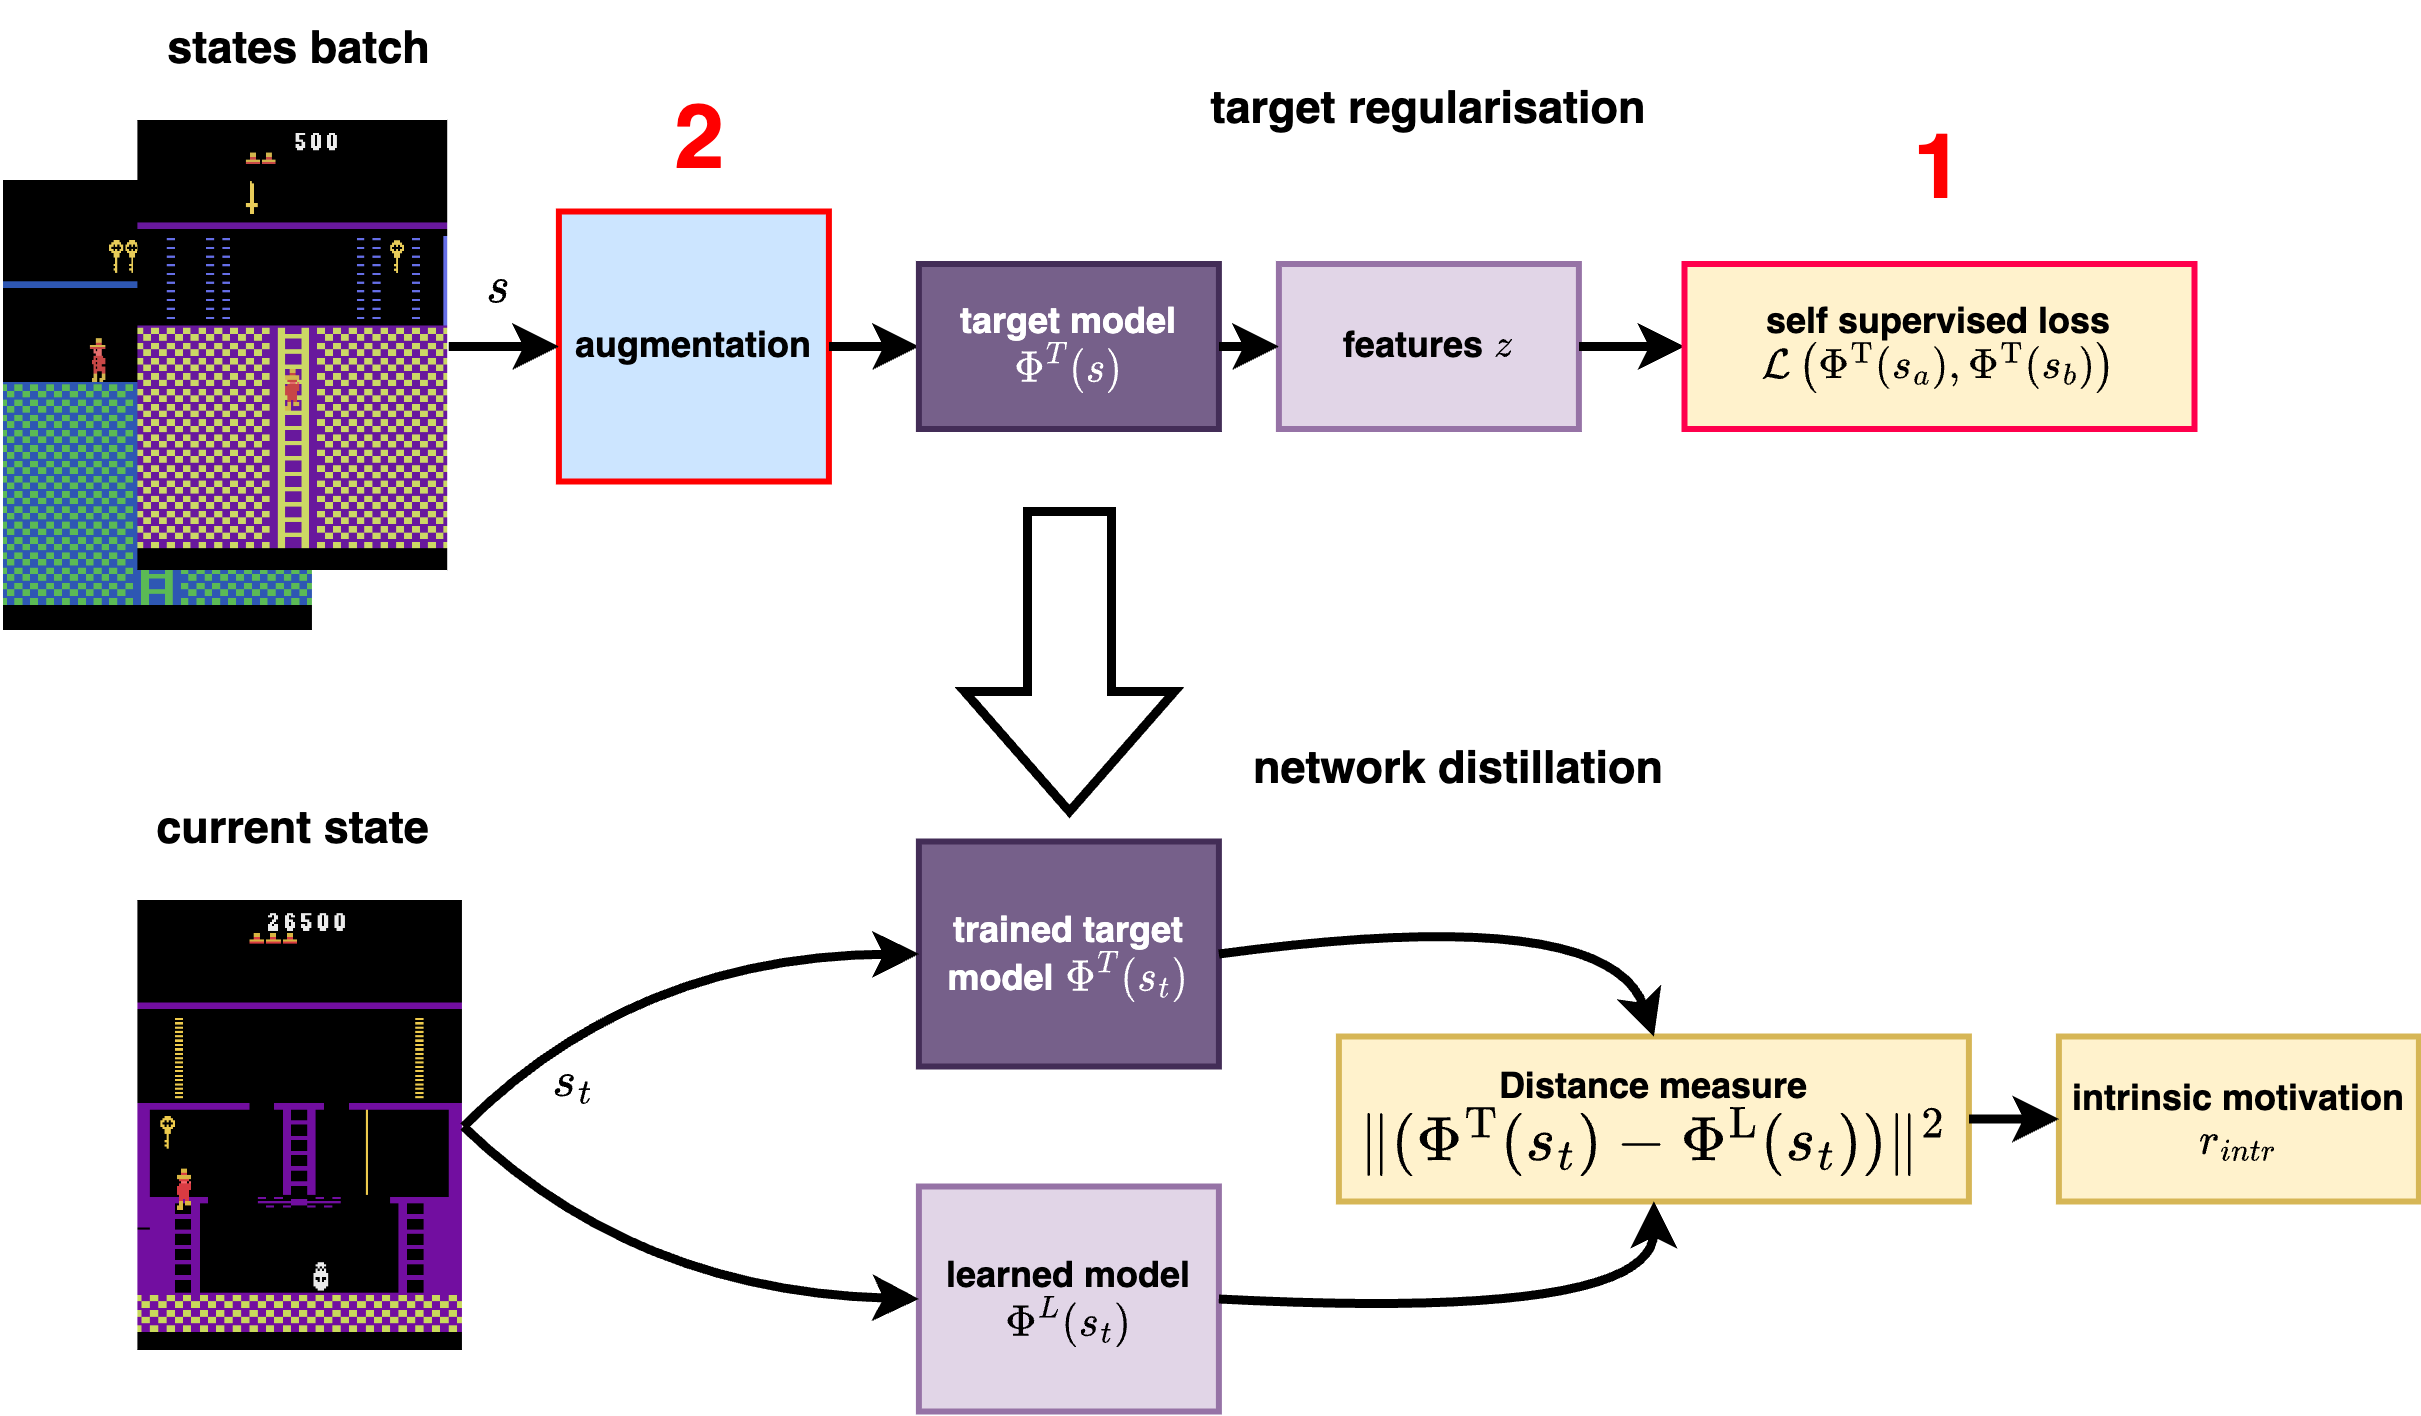
\includegraphics[scale=0.4]{../diagrams/cnd/cnd-cnd-2.png}

\end{frame}

\begin{frame}
  \frametitle{Exploration by self supervised-exploitation}

  \begin{itemize}
    \item we extended existing idea of Random Network Distillation
    \item {\color{red} 1 : } for target model, self supervised training is used
    \item {\color{red} 2 : } augmented states are used to train target model
    \item {\color{red} 3 : } target model is used as distillation source
  \end{itemize} 

  \vskip 0pt plus 1filll
    \centering
    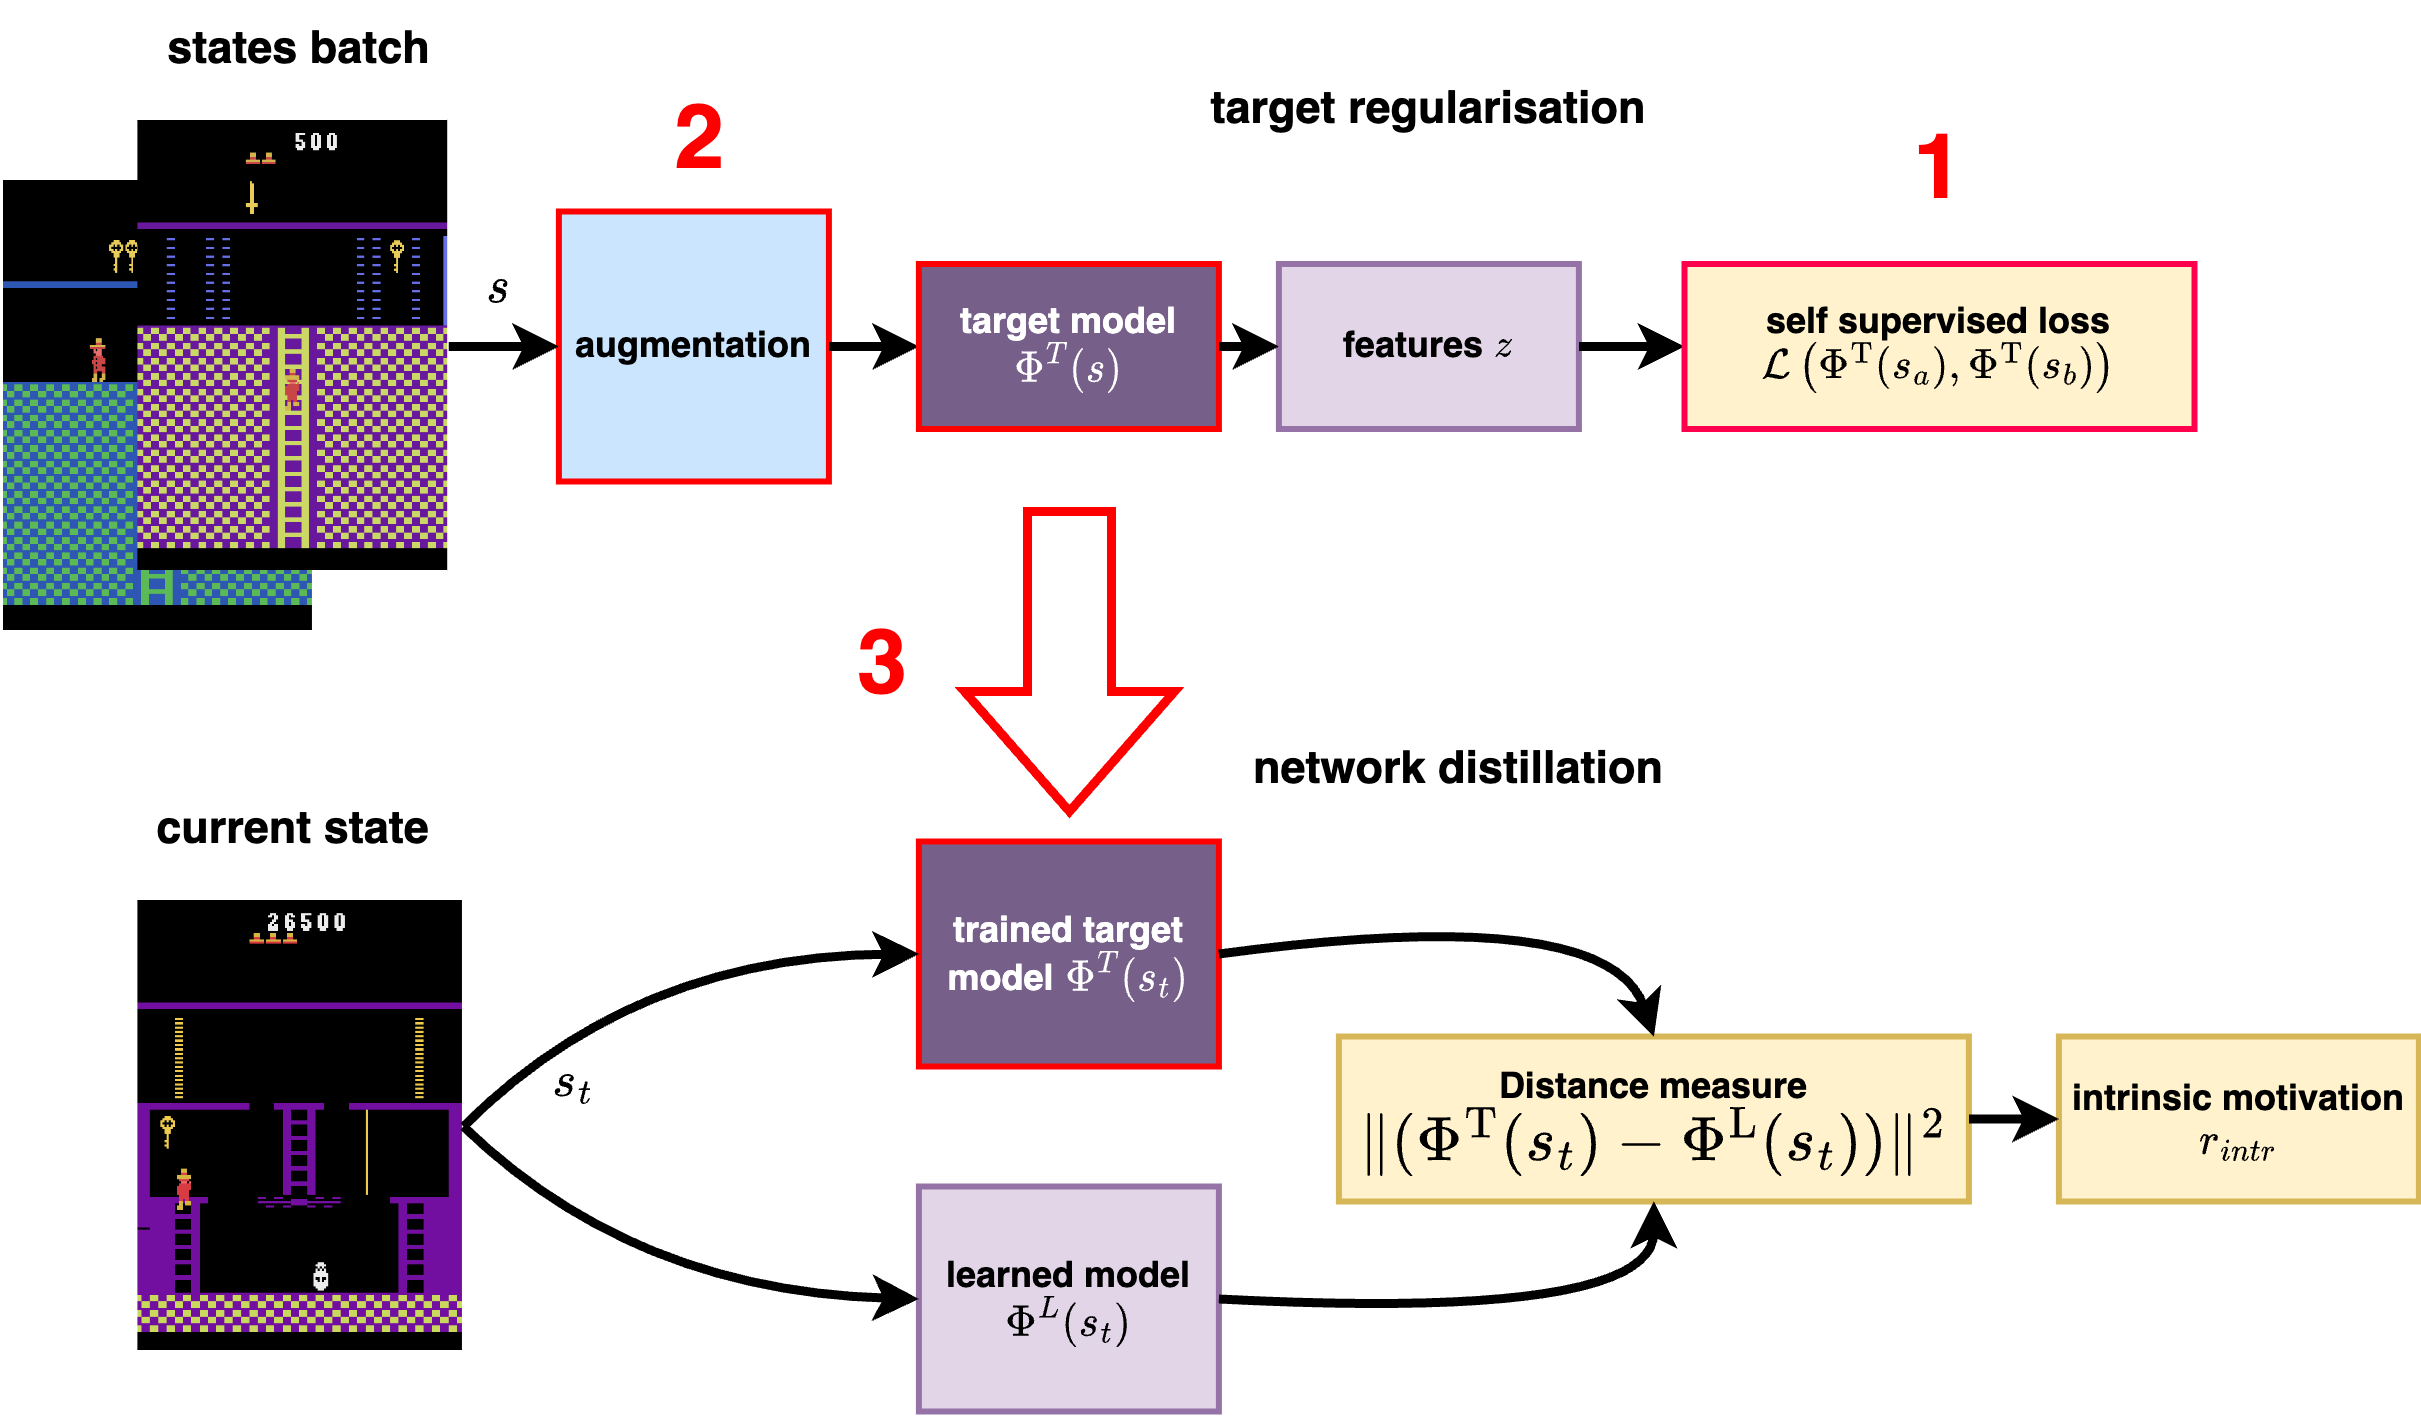
\includegraphics[scale=0.4]{../diagrams/cnd/cnd-cnd-3.png}

\end{frame}

\begin{frame}
  \frametitle{Exploration by self supervised-exploitation}

  \begin{itemize}
    \item we extended existing idea of Random Network Distillation
    \item {\color{red} 1 : } for target model, self supervised training is used
    \item {\color{red} 2 : } augmented states are used to train target model
    \item {\color{red} 3 : } target model is used as distillation source
    \item {\color{red} 4 : } distillation error is used for intrinsic motivation
  \end{itemize} 

  \vskip 0pt plus 1filll 
    \centering
    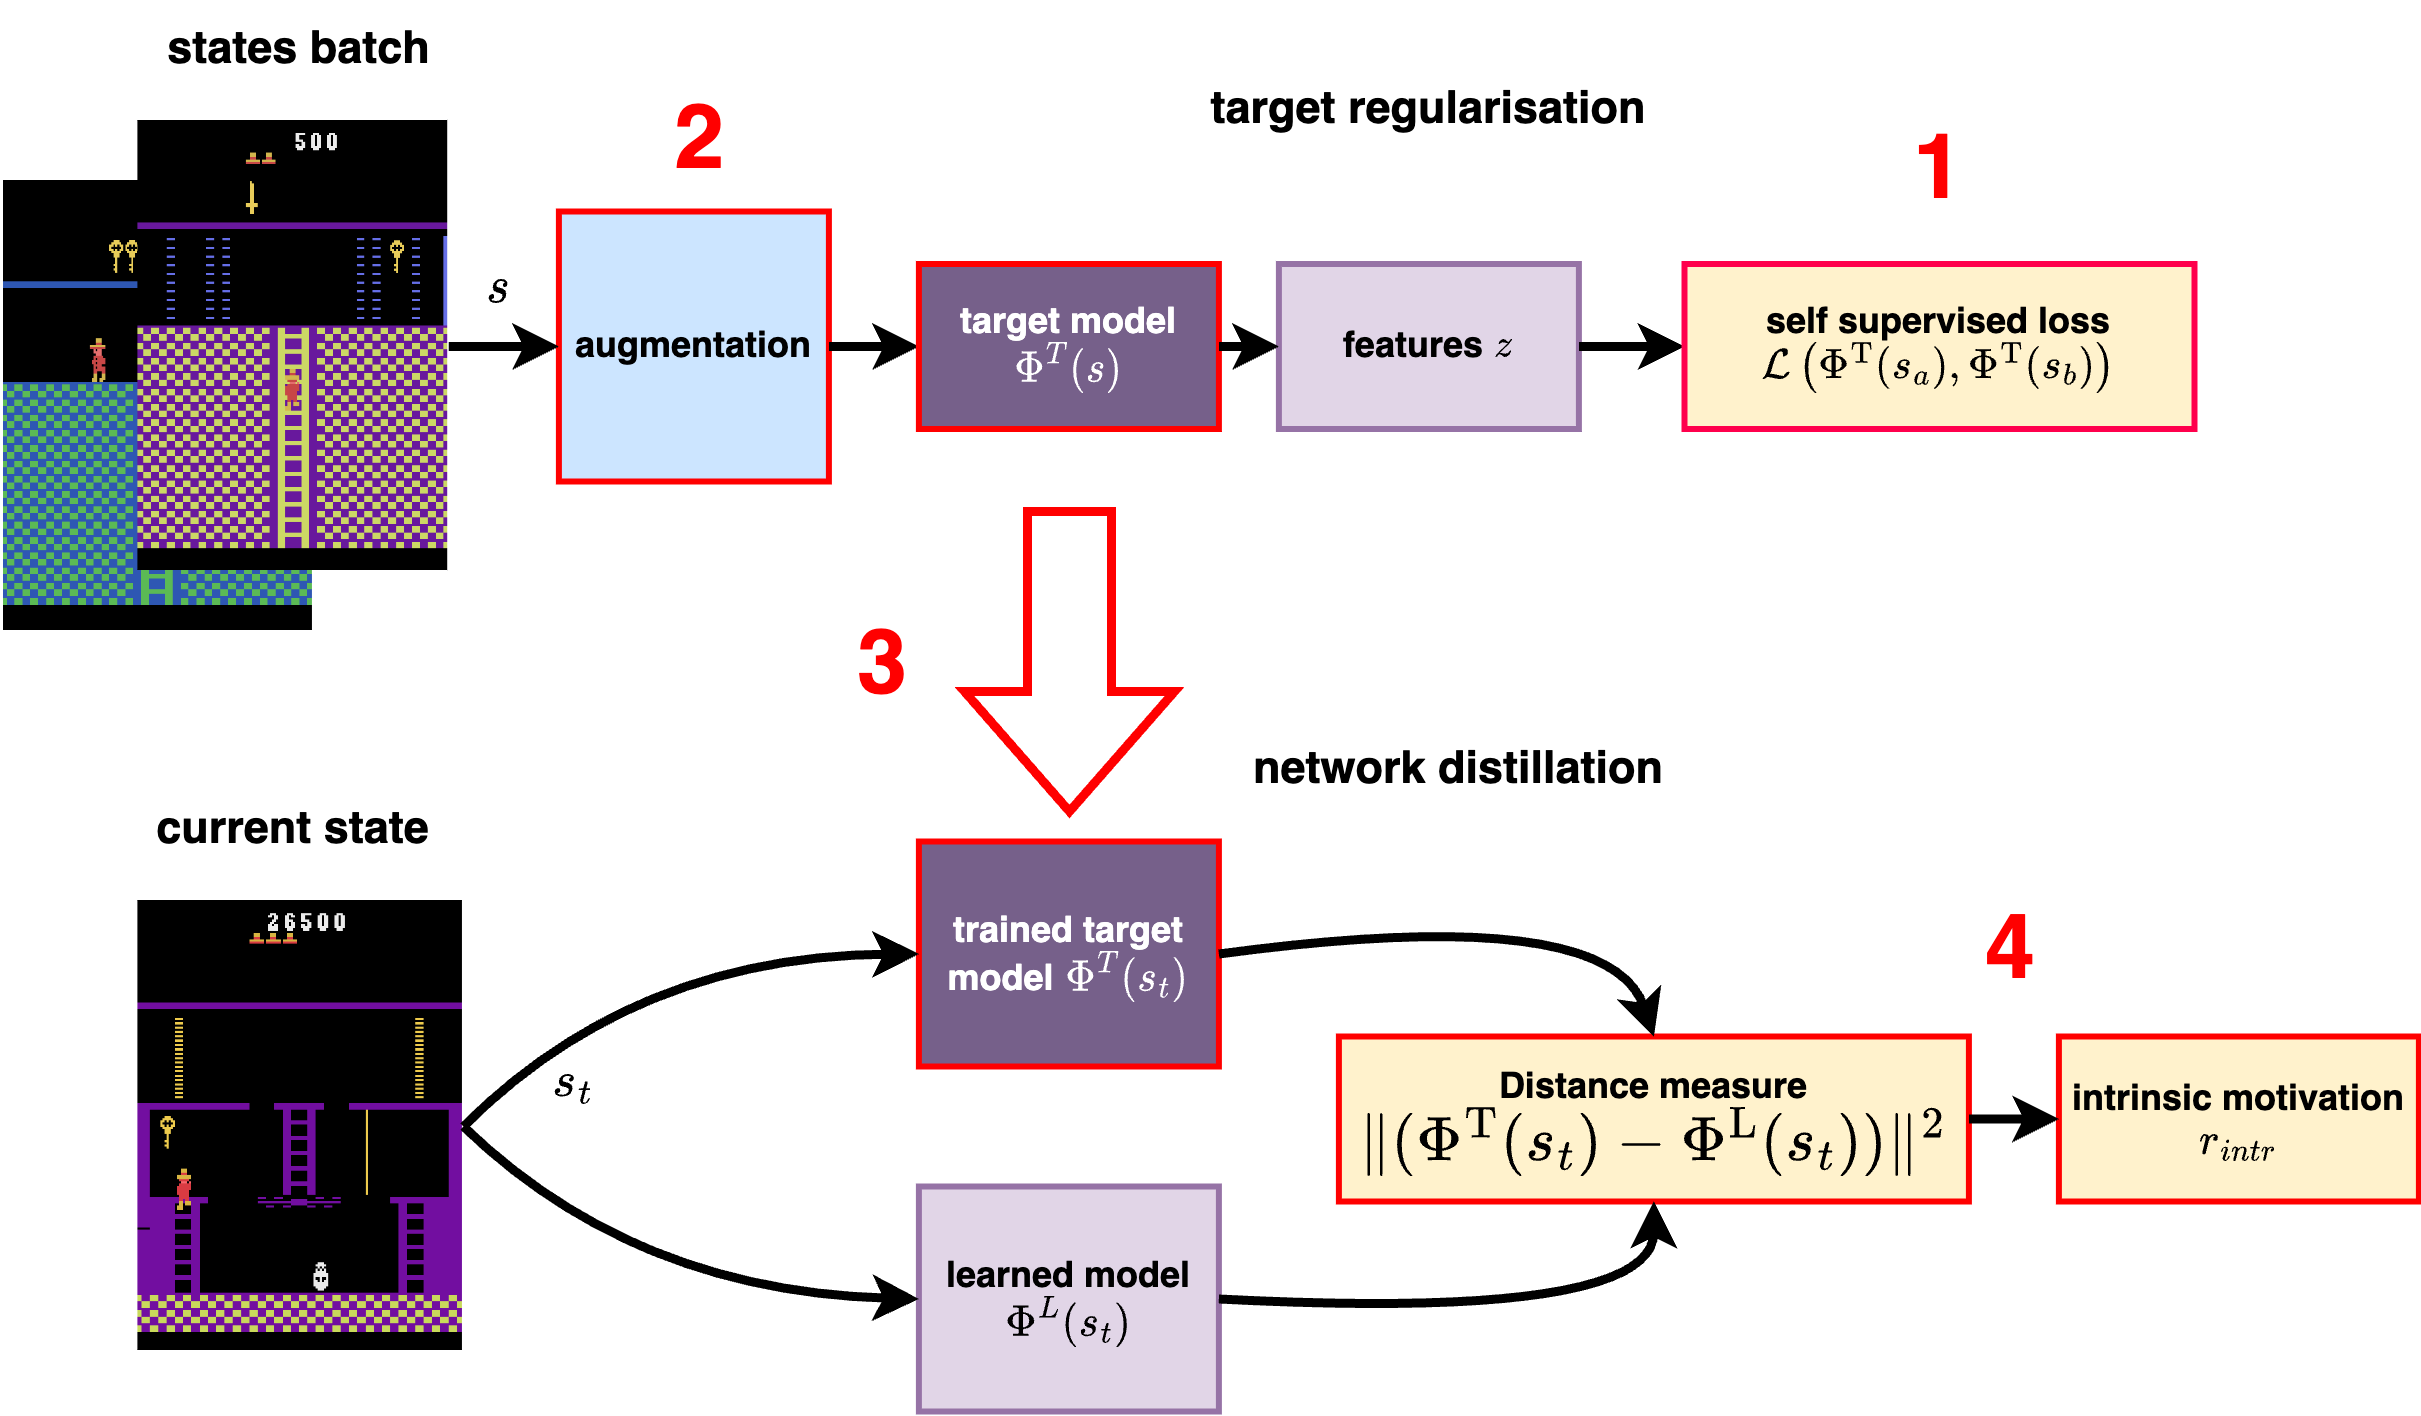
\includegraphics[scale=0.4]{../diagrams/cnd/cnd-cnd-4.png}

\end{frame}


\begin{frame}
  \frametitle{Trained features}
  
  \begin{itemize}
    \item t-SNE features projection for random and trained models
  \end{itemize} 

  \vskip 0pt plus 1filll 
  \begin{columns}
  
    \begin{column}{0.5\textwidth}
      random features
      \bigskip
      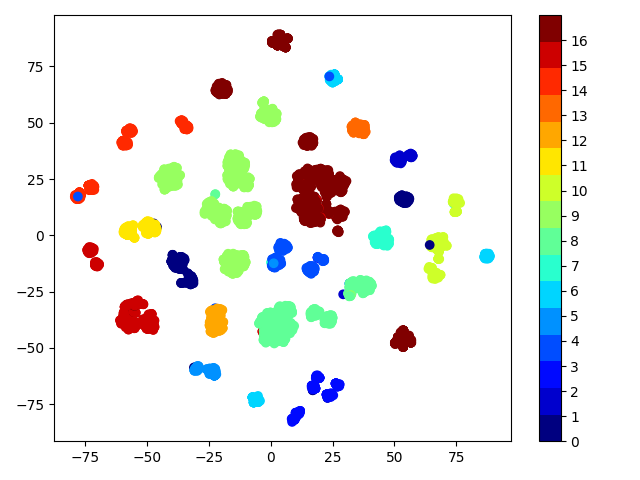
\includegraphics[scale=0.35]{../images/cnd_random.png}
    \end{column}

    \begin{column}{0.5\textwidth}
      self supervised trained features
      \bigskip
      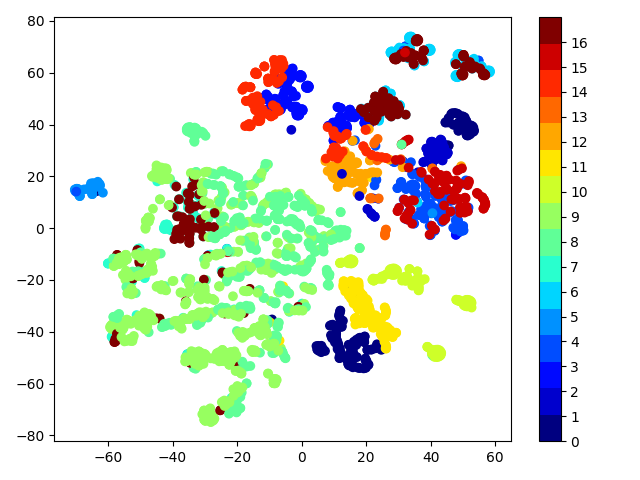
\includegraphics[scale=0.35]{../images/cnd_trained.png}
    \end{column}
  
  \end{columns}
  
\end{frame}

\begin{frame}
  \frametitle{Trained features}
  
  \begin{itemize}
    \item t-SNE features projection for random and trained models
    \item color represents different rooms in Atari Montezuma's Revenge 
  \end{itemize} 

  \vskip 0pt plus 1filll 
  \begin{columns}
  
    \begin{column}{0.5\textwidth}
      random features
      \bigskip
      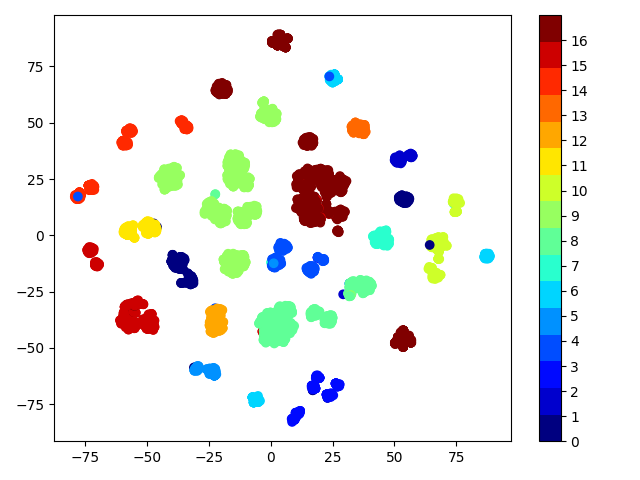
\includegraphics[scale=0.35]{../images/cnd_random.png}
    \end{column}

    \begin{column}{0.5\textwidth}
      self supervised trained features
      \bigskip
      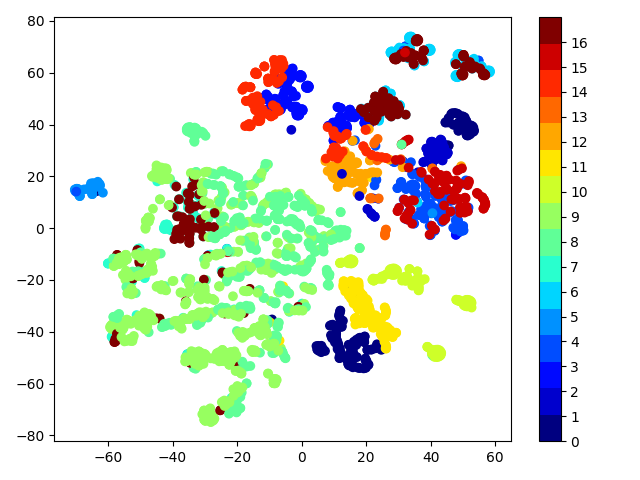
\includegraphics[scale=0.35]{../images/cnd_trained.png}
    \end{column}
  
  \end{columns}
  
\end{frame}




\begin{frame}
  \frametitle{Trained features}

  \begin{itemize}
    \item t-SNE features projection for random and trained models
    \item color represents different rooms in Atari Montezuma's Revenge 
    \item self supervised features provides much bigger variance
    \item preventing agent to stuck
  \end{itemize} 
  
  \vskip 0pt plus 1filll 
  \begin{columns}
  
    \begin{column}{0.5\textwidth}
      random features
      \bigskip
      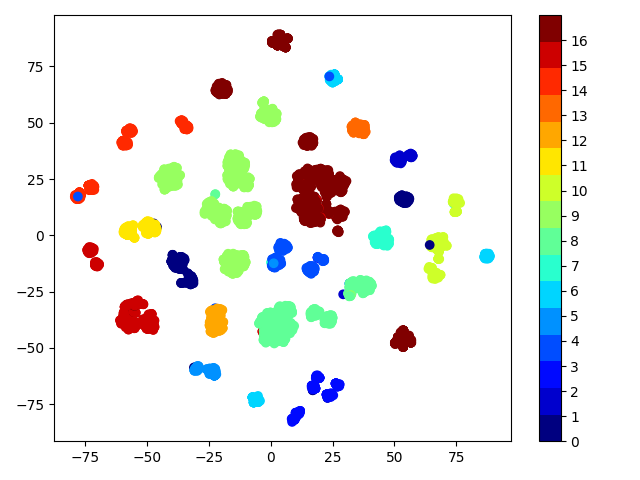
\includegraphics[scale=0.35]{../images/cnd_random.png}
    \end{column}

    \begin{column}{0.5\textwidth}
      self supervised trained features
      \bigskip
      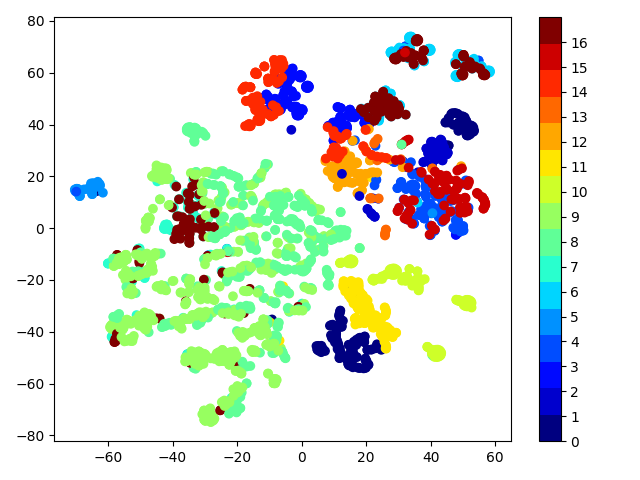
\includegraphics[scale=0.35]{../images/cnd_trained.png}
    \end{column}
  
  \end{columns}
  
\end{frame}


\begin{frame}
  \frametitle{Exploration signal}
  
  \begin{itemize}
    \item Random Network Distillation signal decrease over time
  \end{itemize} 

  \vskip 0pt plus 1filll 
  {\Large Random Network Distillation} \\
  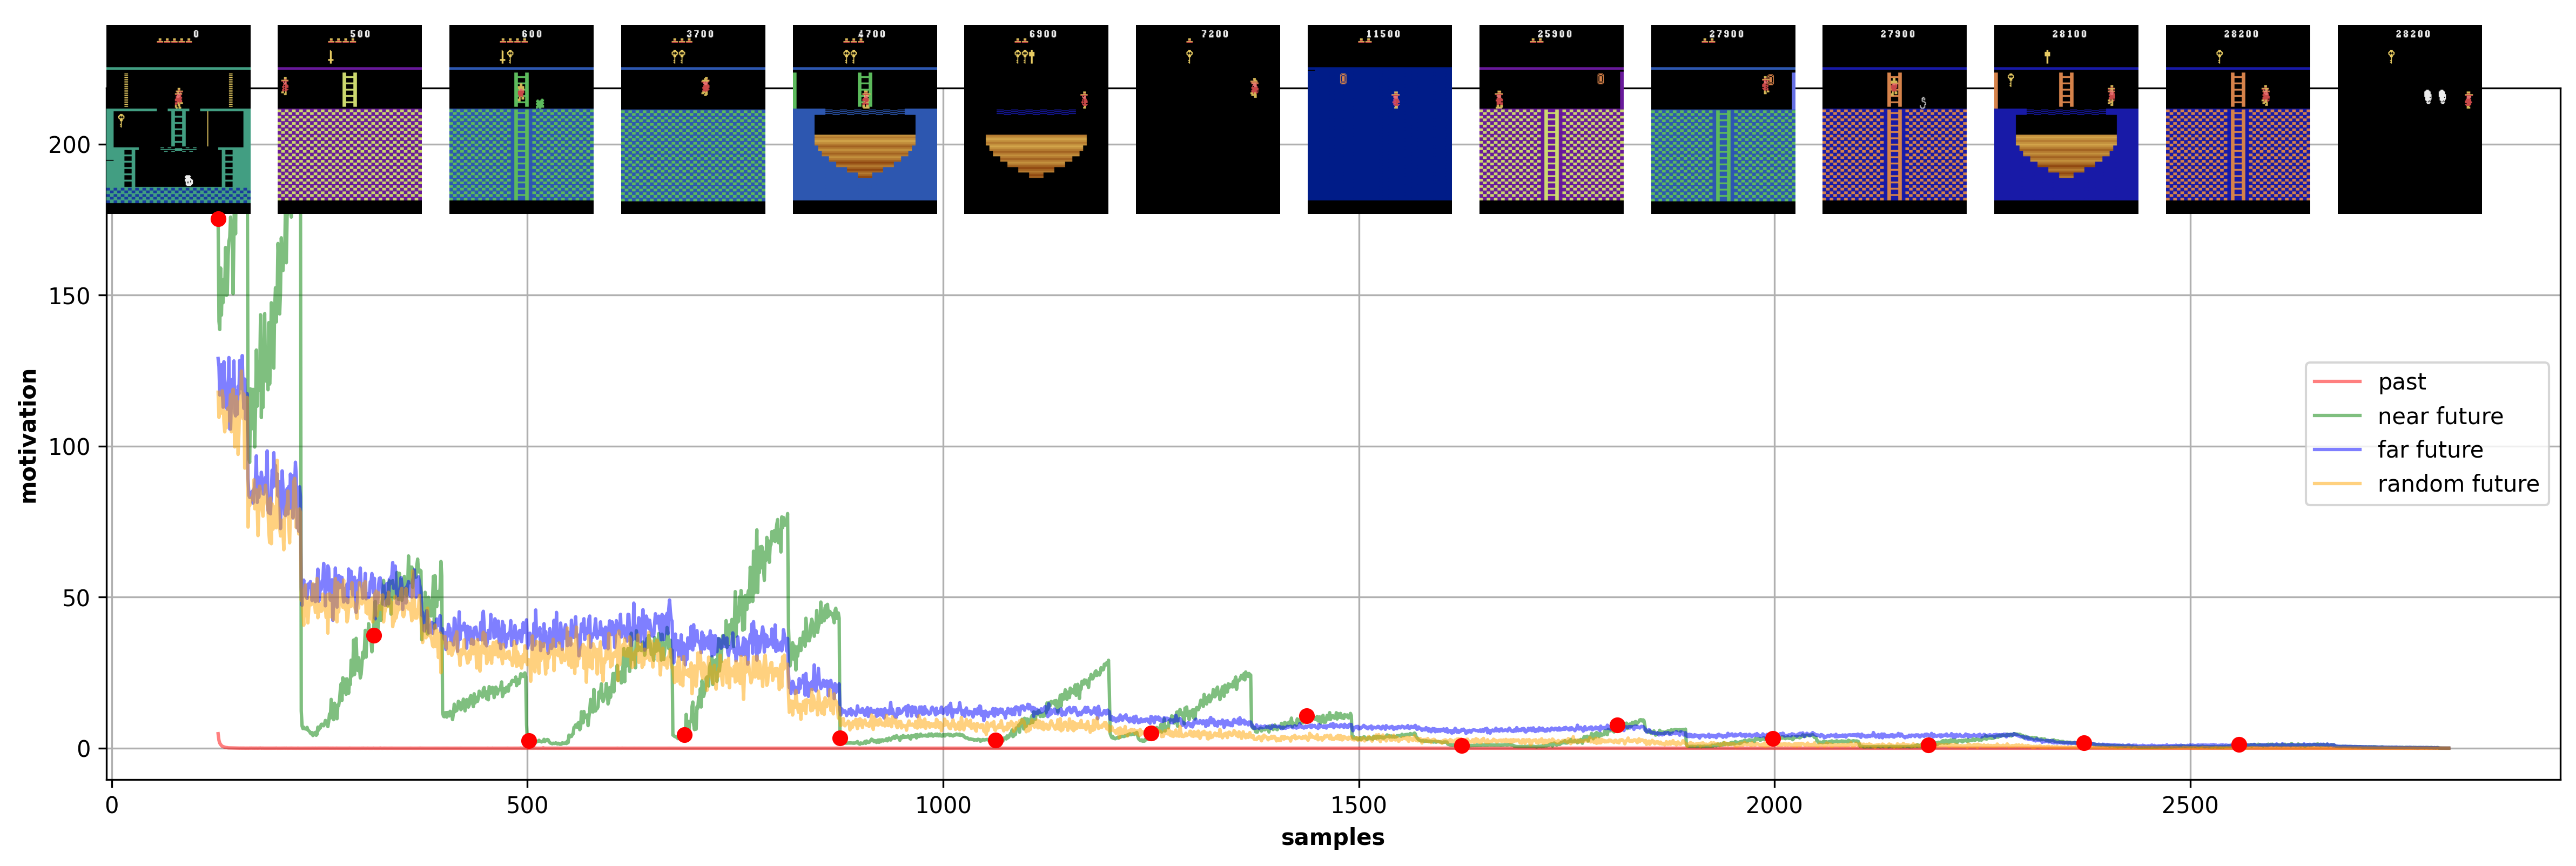
\includegraphics[scale=0.2]{../results/novelty_detection/rnd_result_summary.png}
  \\
  {\Large our method} \\
  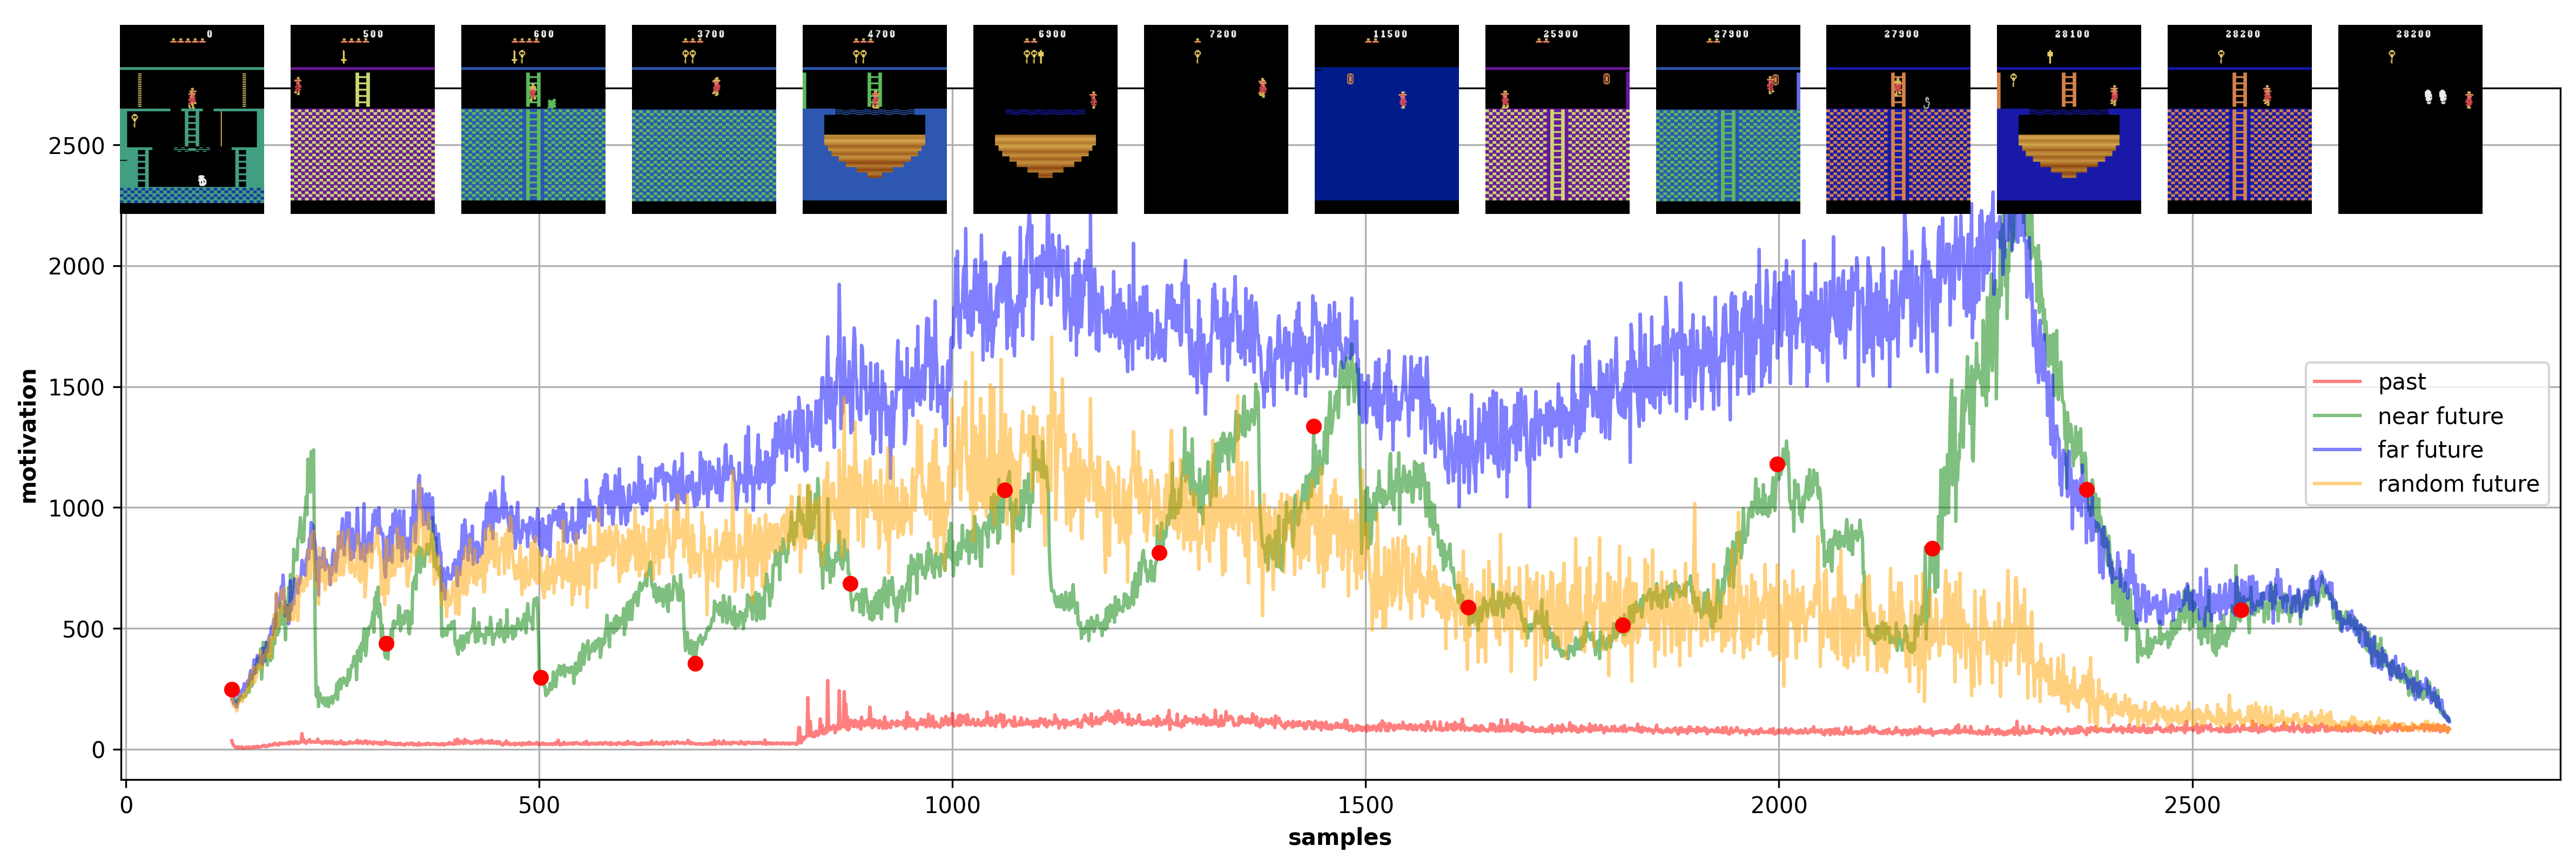
\includegraphics[scale=0.2]{../results/novelty_detection/cnd_vicreg_result_summary.png}

\end{frame}


\begin{frame}
  \frametitle{Exploration signal}
  
  \begin{itemize}
    \item Random Network Distillation signal decrease over time
    \item our method provides more informative signal
  \end{itemize} 
  
  \vskip 0pt plus 1filll 
  {\Large Random Network Distillation} \\
  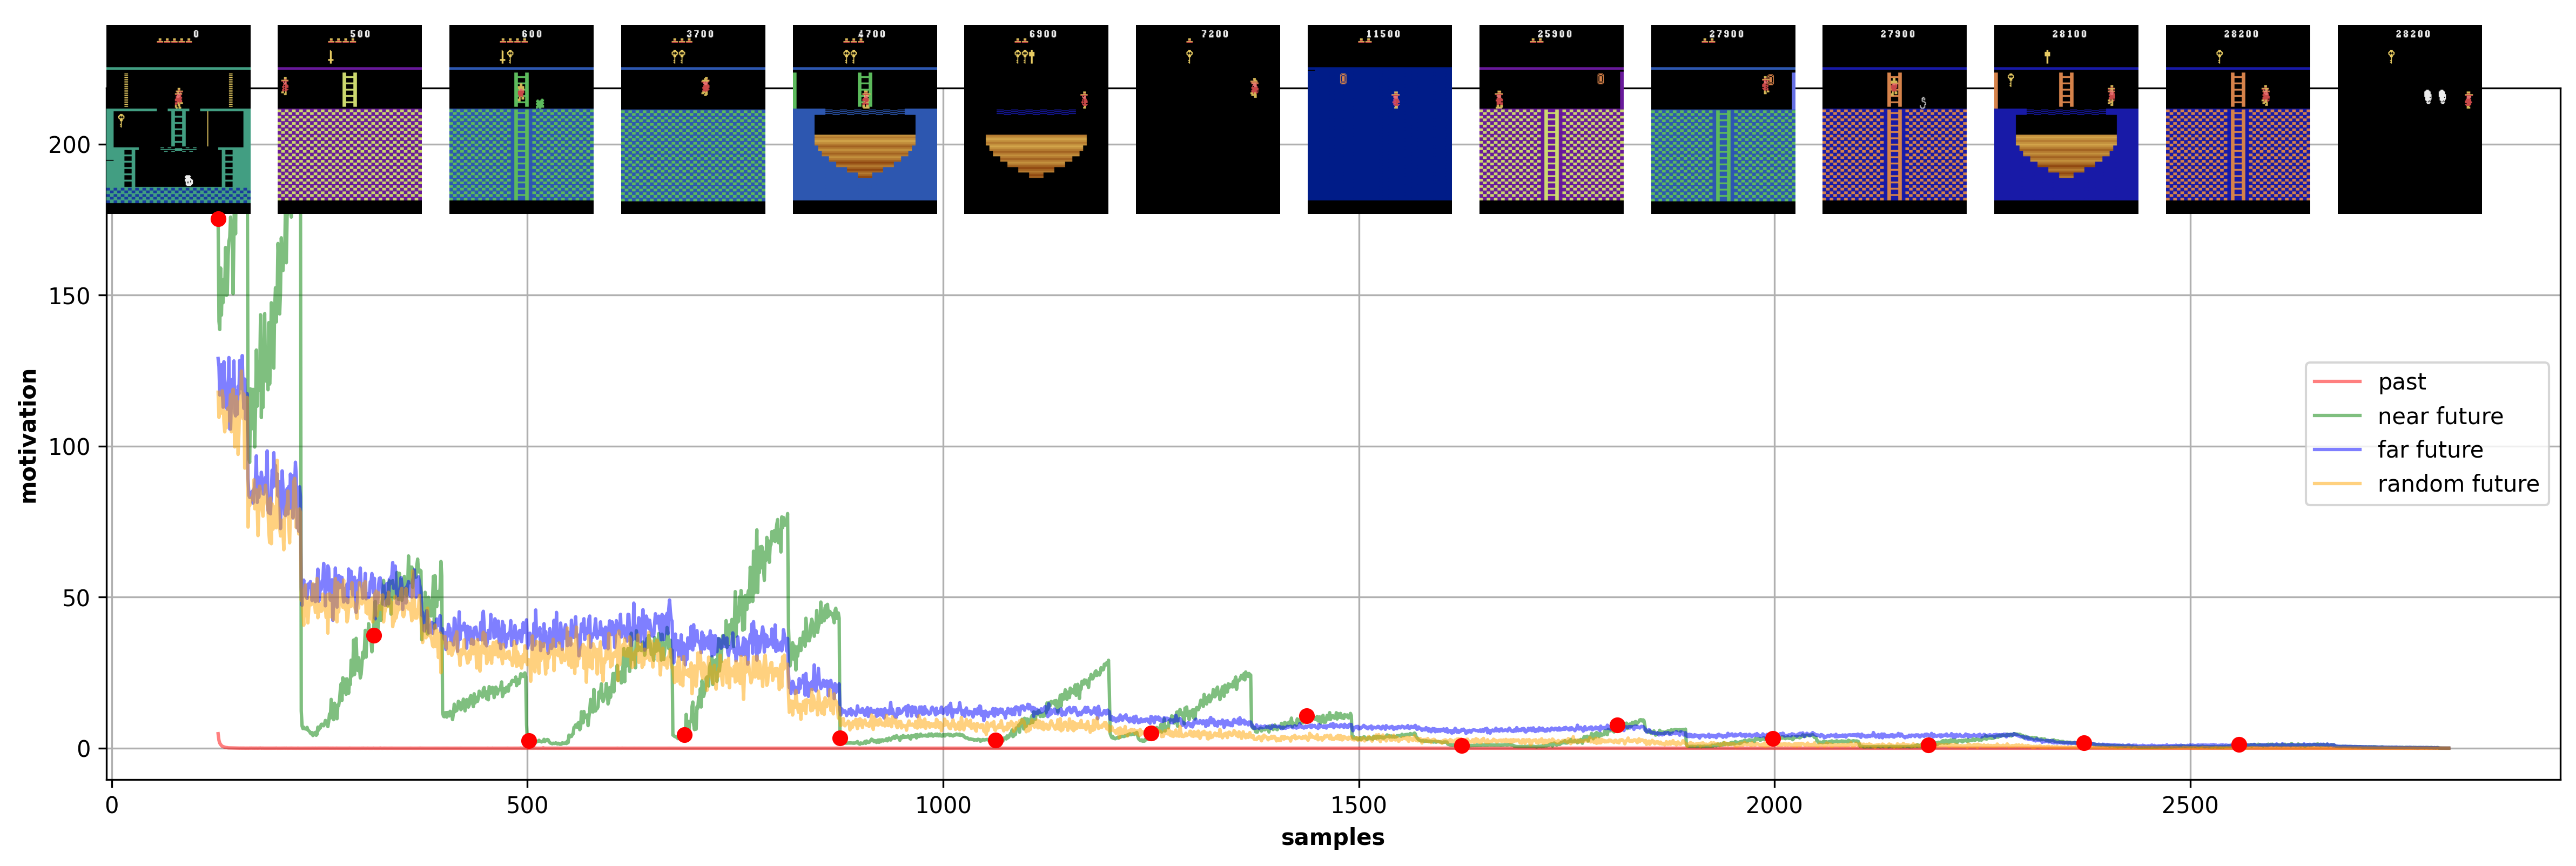
\includegraphics[scale=0.2]{../results/novelty_detection/rnd_result_summary.png}
  \\
  {\Large our method} \\
  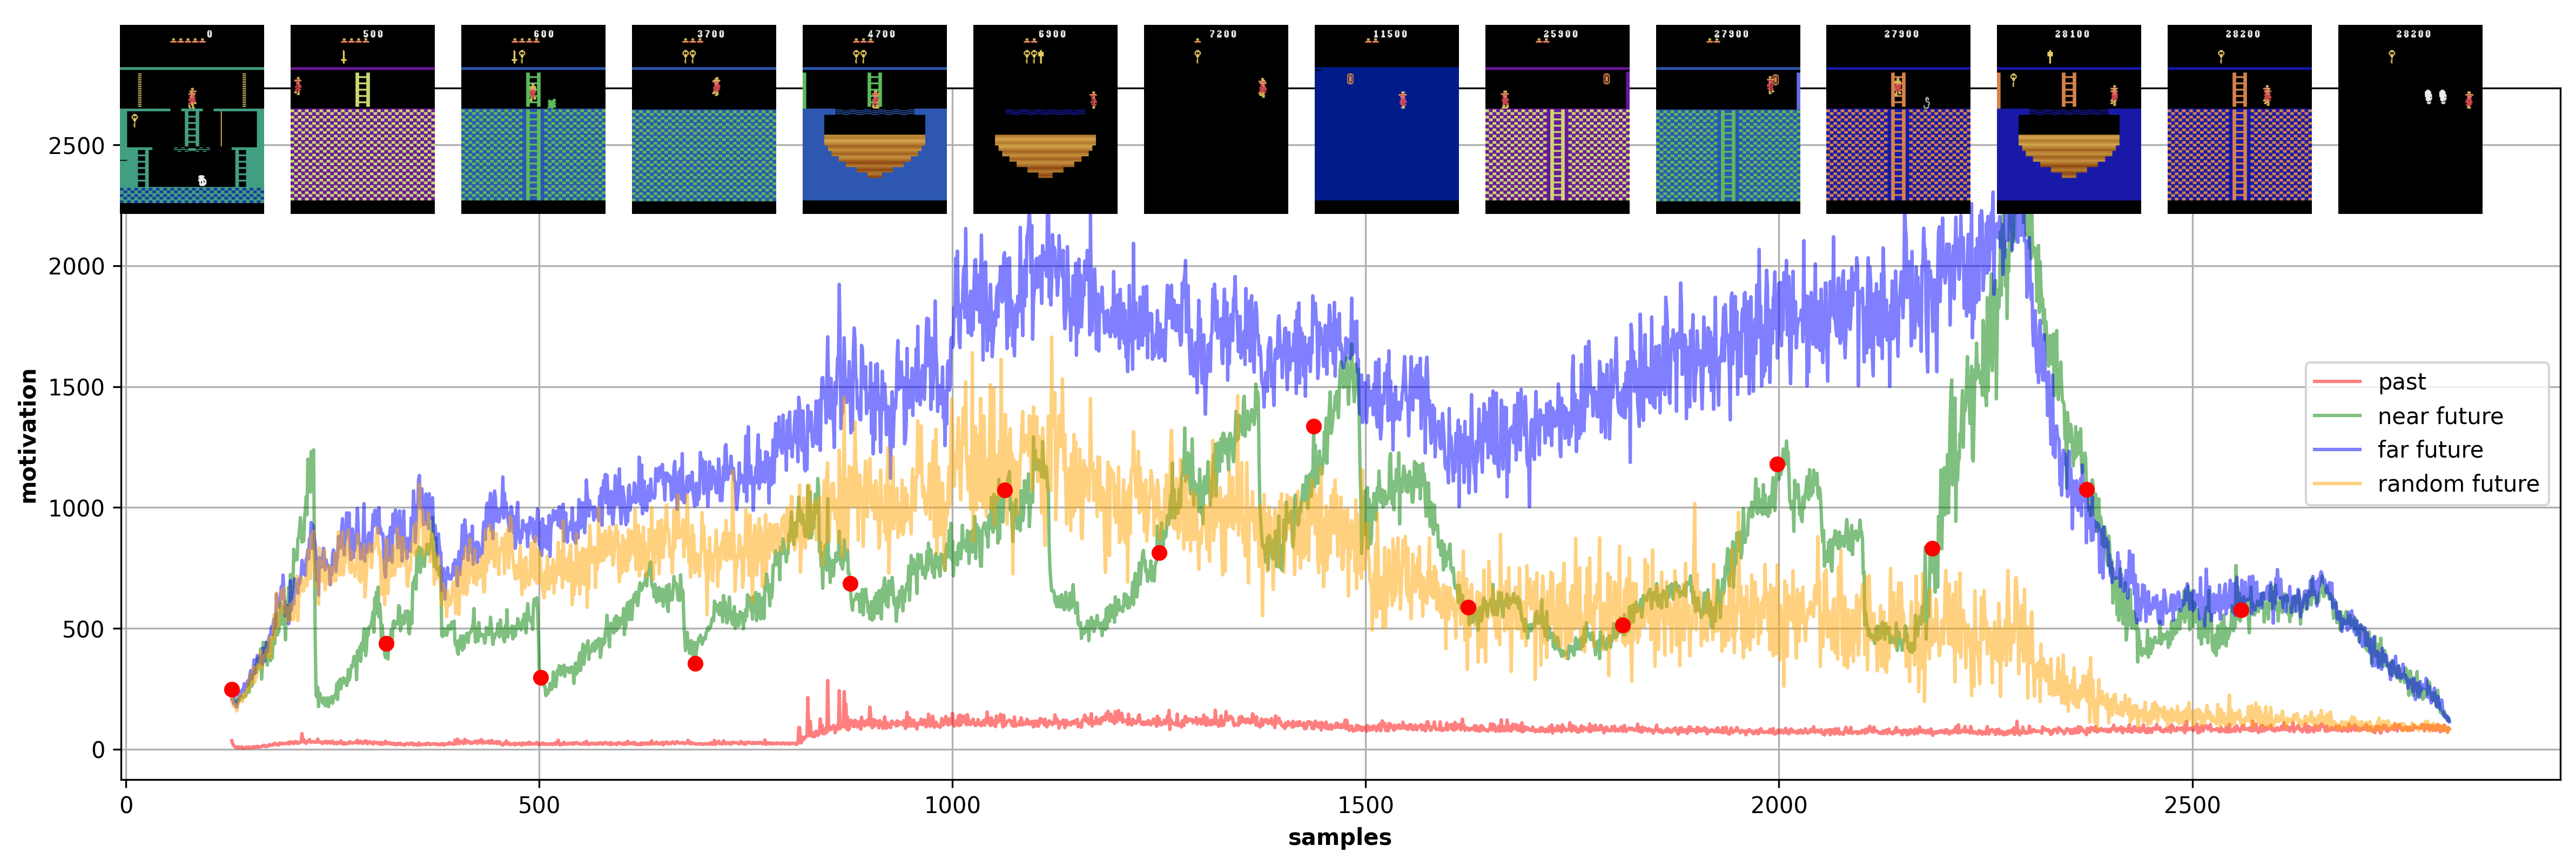
\includegraphics[scale=0.2]{../results/novelty_detection/cnd_vicreg_result_summary.png}

\end{frame}


\begin{frame}
  \frametitle{Results}

  \begin{itemize}
    \item Montezuma's Revenge, with score {\color{red}25 000+}
    \item Private Eye, with score {\color{red}12 000+}
    \item Venture, Gravitar 
    \item 128M samples total - only single GPU needed
  \end{itemize} 
  
  
  \begin{columns}
  
    \begin{column}{0.5\textwidth}
      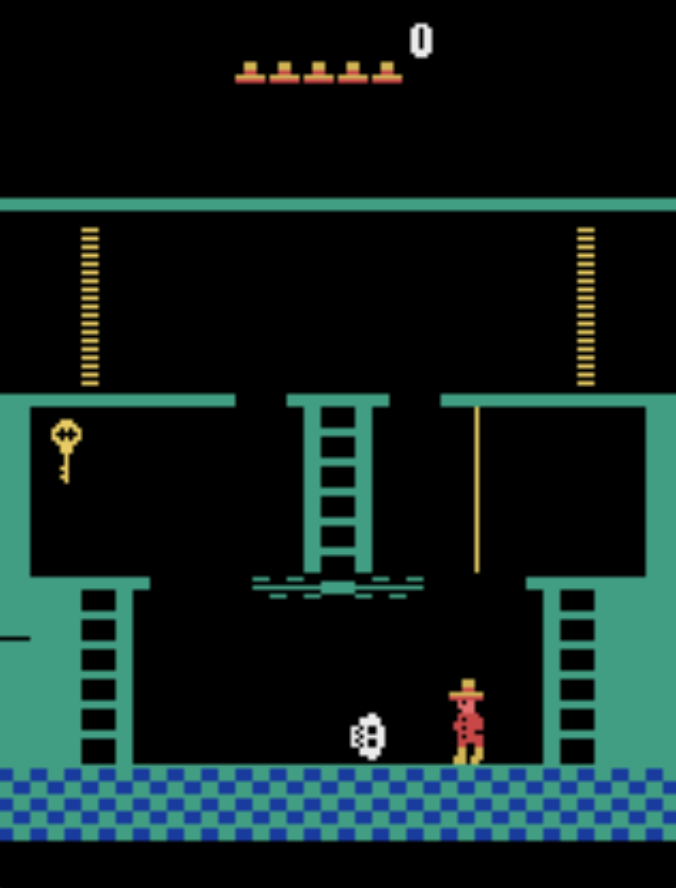
\includegraphics[scale=0.32]{../images/montezuma.png}
    \end{column}

    \begin{column}{0.5\textwidth}
      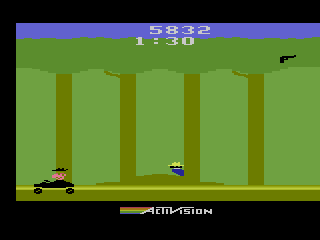
\includegraphics[scale=0.4]{../images/privateeye.png}
    \end{column}
  
  \end{columns}

\end{frame}

\begin{frame}
  video of playing agent
\end{frame}



\begin{frame}
  \frametitle{Results}
  
  {\Large solved Procgen hard exploration seeds} \\
  environments : Caveflyer, Climber, Coinrun, Jumper
  
  \begin{columns}
  
    \begin{column}{0.6\textwidth}
      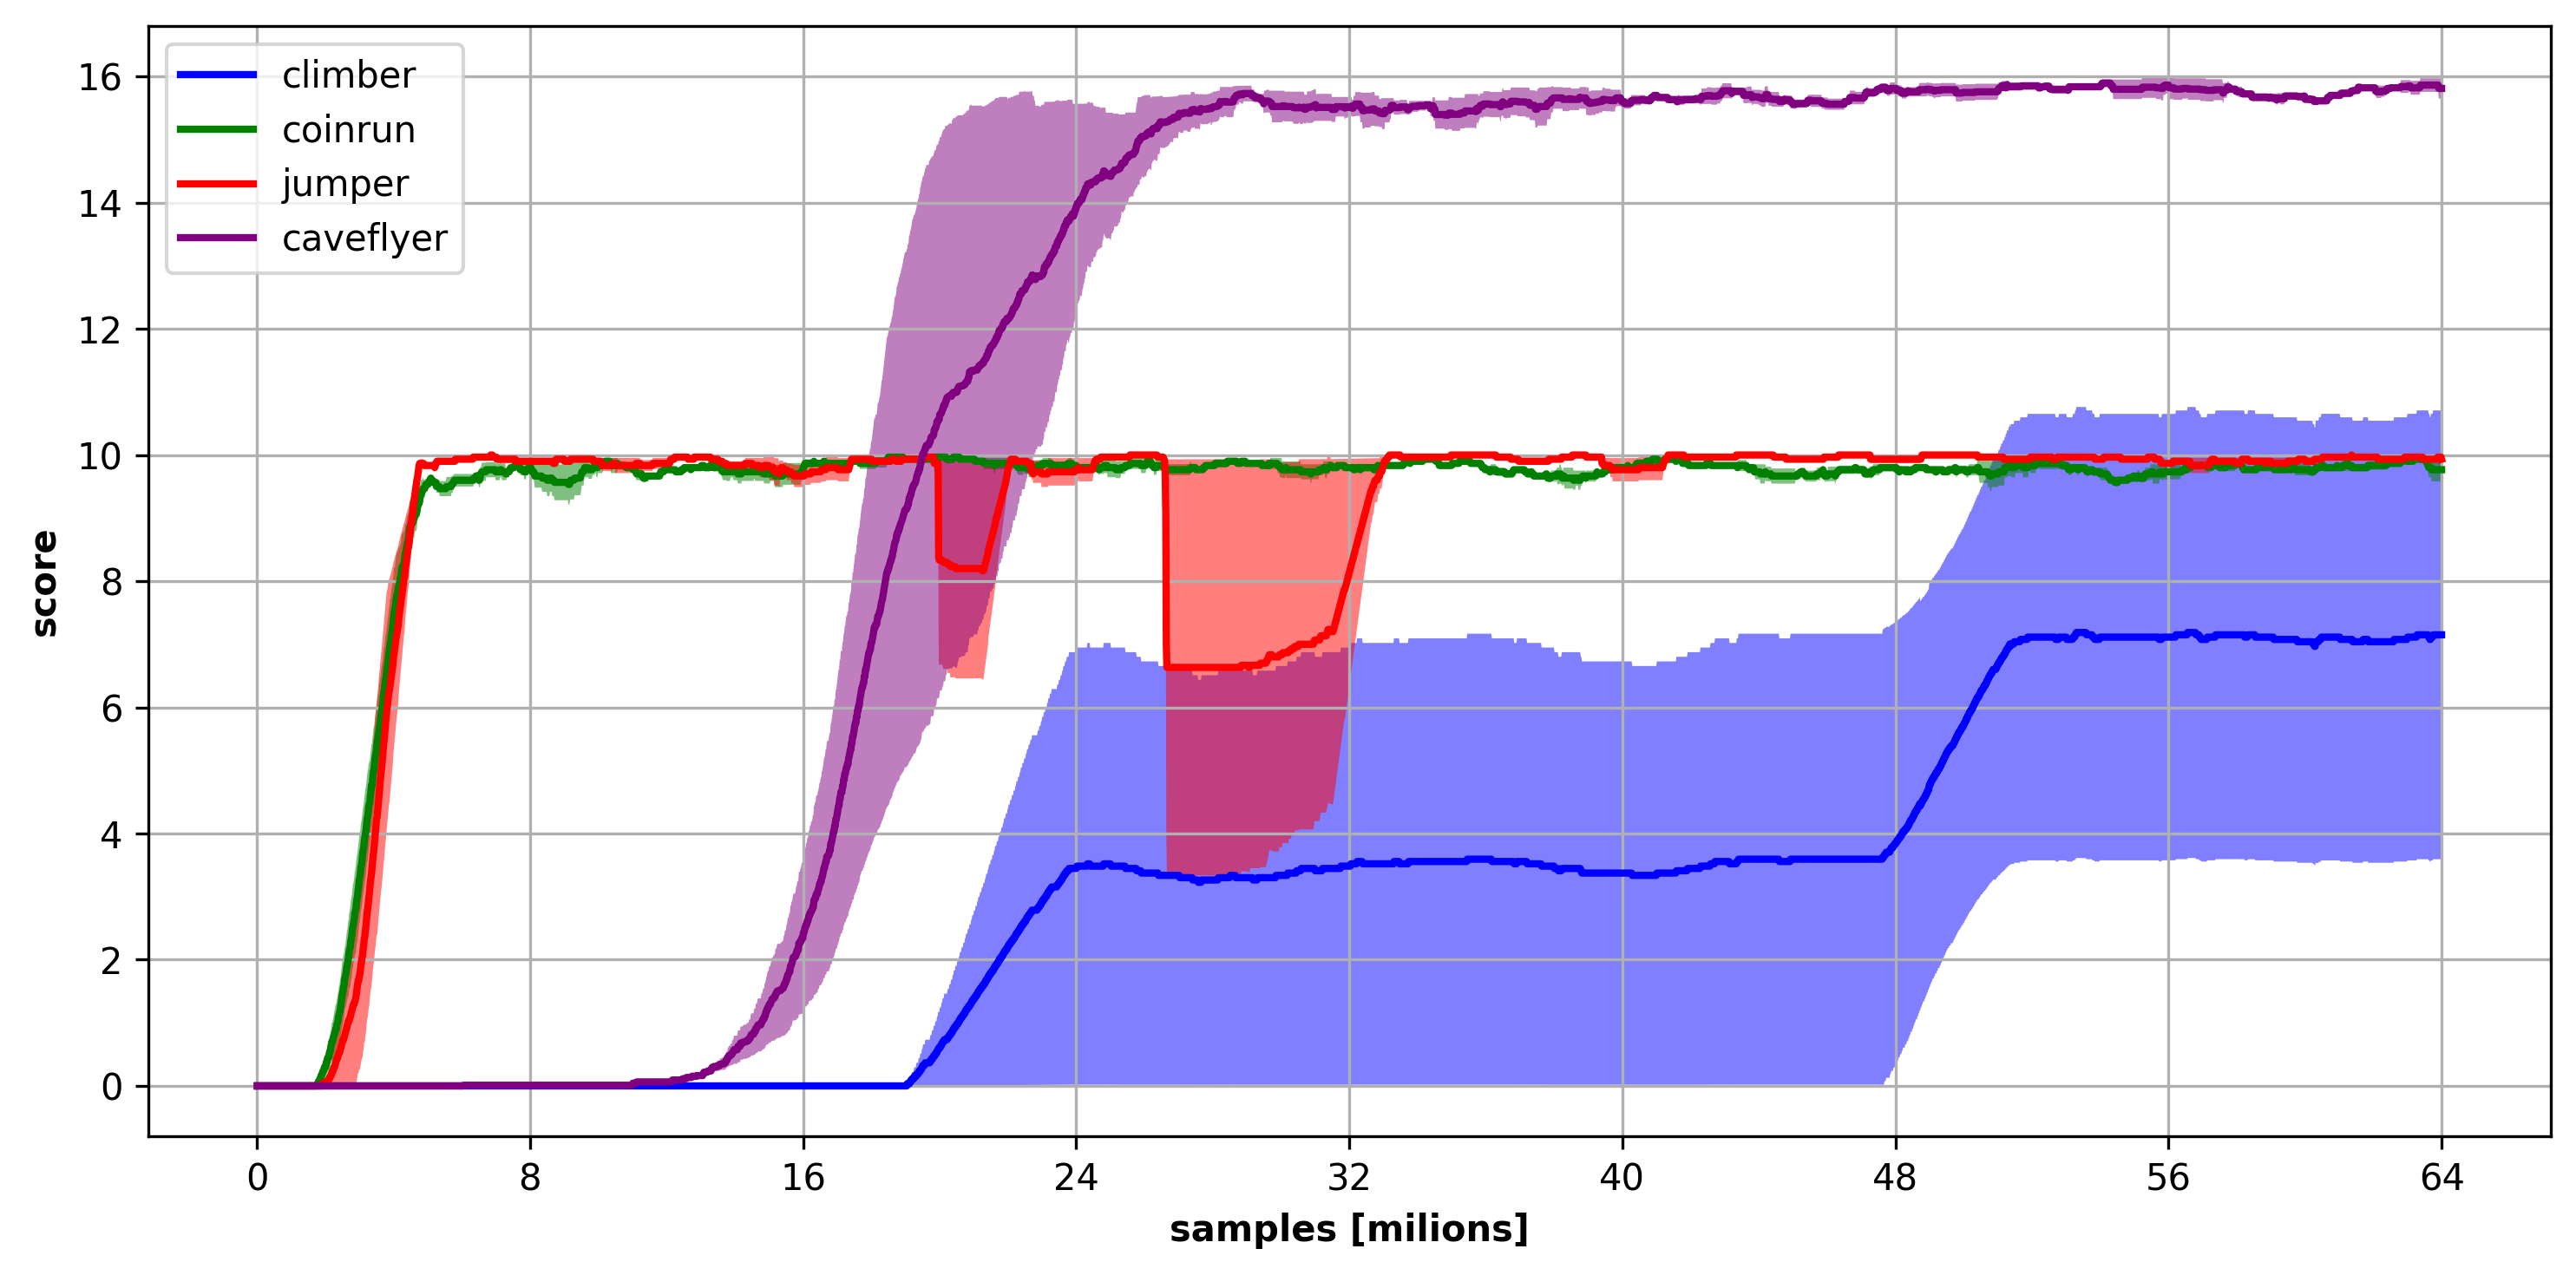
\includegraphics[scale=0.25]{../results/summary/procgen_all_score.png}
    \end{column}

    \begin{column}{0.4\textwidth}
      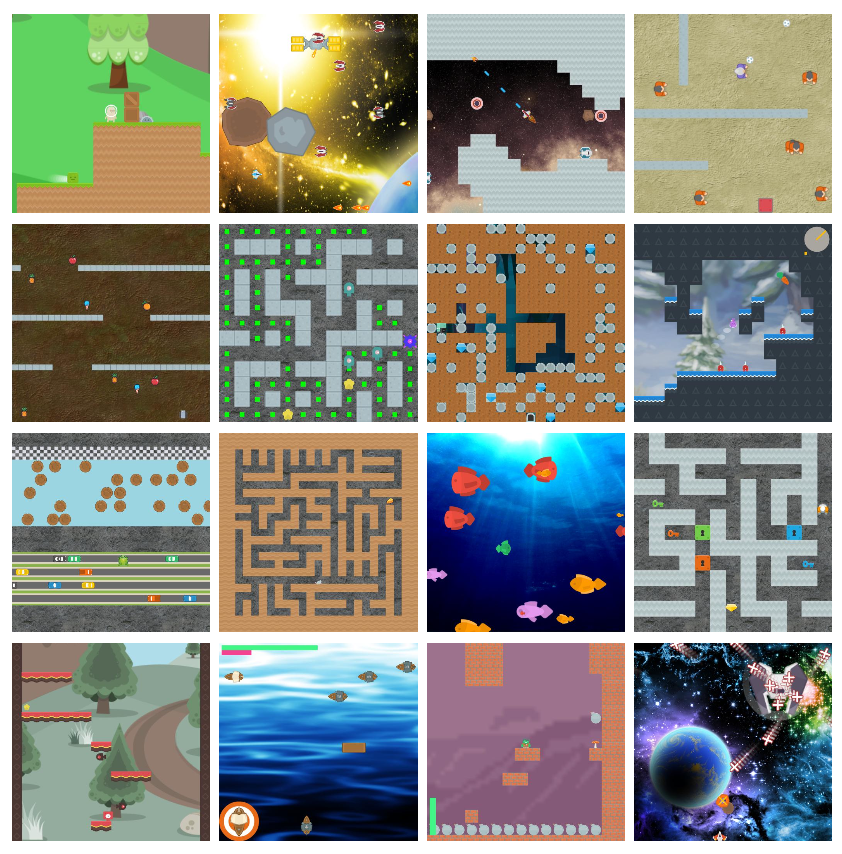
\includegraphics[scale=0.25]{../images/procgen.png}
    \end{column}
  
  \end{columns}

\end{frame}

\begin{frame}
  video of playing agent
\end{frame}



\begin{frame}
  \frametitle{Summary}

  \begin{itemize}
    \item{New sample efficient exploration method}
    \item{Novel view to features z-spaces}
    \item{solved environments : \\ Procgen (Climber, Caveflyer, Coinrun, Jumper) \\ Atari (Montezuma, Solaris, Private Eye, Venture, Gravitar)}
    \item{github sources : {\footnotesize \\ \url{https://github.com/Iskandor/MotivationModels} \\ \url{https://github.com/michalnand/reinforcement_learning}}}
  \end{itemize}
  
  
\end{frame}


\end{document}